\documentclass[12pt]{article}

\usepackage{amssymb,amsmath,amsfonts,eurosym,geometry,ulem,graphicx,caption,color,setspace,sectsty,comment,footmisc,caption,pdflscape,subfigure,array,hyperref,enumitem}
\usepackage[round]{natbib}

\normalem

\onehalfspacing
\newtheorem{theorem}{Theorem}
\newtheorem{lemma}{Lemma}
\newtheorem{corollary}[theorem]{Corollary}
\newtheorem{proposition}{Proposition}
\newenvironment{proof}[1][Proof of]{\noindent\textbf{#1} }{\ \rule{0.5em}{0.5em}}

% \newtheorem{hyp}{Hypothesis}
% \newtheorem{subhyp}{Hypothesis}[hyp]
% \renewcommand{\thesubhyp}{\thehyp\alph{subhyp}}

% \newcommand{\red}[1]{{\color{red} #1}}
% \newcommand{\blue}[1]{{\color{blue} #1}}


% \newcolumntype{L}[1]{>{\raggedright\let\newline\\arraybackslash\hspace{0pt}}m{#1}}
% \newcolumntype{C}[1]{>{\centering\let\newline\\arraybackslash\hspace{0pt}}m{#1}}
% \newcolumntype{R}[1]{>{\raggedleft\let\newline\\arraybackslash\hspace{0pt}}m{#1}}

\geometry{left=1.0in,right=1.0in,top=1.0in,bottom=1.0in}
\graphicspath{images/}

\begin{document}

\begin{titlepage}
\title{Employee Referral Programs: Always good?\thanks{abc}}
\author{Georgii Aleksandrov\thanks{abc}}
\date{\today}
\maketitle
\begin{abstract}
\noindent Abstract here\\
\vspace{0in}\\
\noindent\textbf{Keywords:} employee referrals, employee referral programs, hiring\\
\vspace{0in}\\
%\noindent\textbf{JEL Codes:} key1, key2, key3\\

\bigskip
\end{abstract}
\setcounter{page}{0}
\thispagestyle{empty}
\end{titlepage}
\pagebreak \newpage




\doublespacing


\section{Introduction} \label{sec:introduction}

%----------------------
%INTRO - RQ
%----------------------

Based on your discussion and conclusion sections, you can structure your introduction in the following way:
\begin{itemize}
    \item Introduction to the topic: Start with a general introduction to the concept of employee referrals and their significance in the labor market. Highlight the potential benefits of employee referral programs (ERPs) for firms, such as improved candidate quality and reduced hiring costs.
    \item Gap in the literature: Discuss the existing research on labor market referrals and point out the limitations or gaps in the current literature. Emphasize that most previous studies have focused on either voluntary referrals or ERPs, but there is a need to consider both aspects together to gain a comprehensive understanding.
    \item Objective and research question: Clearly state the objective of your study, which is to develop a model of employee referrals that examines the conditions under which the implementation of an ERP is beneficial for firms. Formulate a research question that encompasses the main focus of your investigation.
    \item Assumptions and framework: Provide an overview of the key assumptions on which your model is built, as discussed in your conclusion section. Mention the two types of worker ability, the positive correlation among connected workers' ability levels, and the social preferences of current employees towards their social contacts.
    \item Methodology: Briefly explain the methodology you used to develop the model and analyze the effectiveness of referrals under different labor market conditions. Highlight the importance of incorporating both voluntary referrals and ERPs in the analysis.
    \item Contribution and significance: Discuss the potential contributions of your research to the field. Highlight how your study fills the gap in the literature by providing insights into the combined effects of voluntary referrals and ERPs on firm outcomes. Emphasize the practical implications of your findings for firms and the potential for further empirical research in this area.
    \item Outline of the paper: Provide a brief overview of the structure of your paper, mentioning the main sections or chapters and their respective content.
\end{itemize}

Remember to keep the introduction concise and engaging, capturing the reader's interest and setting the stage for the rest of your paper.

%\section{Literature Review} \label{sec:literature}

\section{Model} \label{sec:model}
This section presents a model of employee referrals, which allows the firm to fill its vacant positions in several ways. In addition to the formal recruitment method of finding candidates from the labor market, the firm can also utilize referrals from its current employees. The model assumes that the production function of the firm depends not only on the general ability of the worker but also on a specific component. This assumption can be interpreted from different perspectives, such as the classical theory of human capital by \cite{becker1962investment}, its modified version by \cite{lazear2009firm}, and the concept of task-specific human capital studied by \cite{gibbons2004task}. Referring employees do not possess additional information about referred candidates' abilities. However, referrals can still benefit employers due to the correlation between the abilities of referred and referring workers. 

%I consider two variants of the model: the first assumes that firms in the labor market cannot separately observe the general and specific abilities of workers, but only their realized output. Later sections relax these assumptions to allow all labor market participants to observe both general and specific abilities.
Following subsections include the model setup, analysis of the model with voluntary referrals, and analysis of the model in which firms can launch employee referral programs with bonuses paid to referring employees if their referrals are hired. 

\subsection{Model setup}
This subsection includes the main assumptions, timing of the model, utilities of employees, and firm profits. The main assumptions of the model are listed below.
\begin{enumerate}[label={A}{\arabic*}.]
	\item Production takes place in firms, and there is free entry into production. Firms in the labor market are assumed to have no market power.
	\item A worker's career lasts for $T = 2$ periods. A worker's labor supply is fixed and inelastic, meaning that the worker cannot adjust the amount of time devoted to work or leisure. The labor supply is fixed at one unit for each worker in every period $t_l = 1,2$.
	\item Both workers and firms are risk neutral and have a discount factor $\delta = 0$. Hence, the wages are determined by spot-market contracting, following the assumption made in \cite{gibbons1999theory} that there are no benefits to long-term contracts in a setting where workers and firms are risk-neutral and have a discount rate of zero. Another assumption taken from \cite{gibbons1999theory} is that wages that are paid in advance of production, as opposed to one-period piece-rate contracts. If a worker is indifferent between accepting the offer of a firm and accepting the offer from the labor market, the worker always chooses the former, following the assumption in \cite{ekinci2016employee}.
    \item The output of a worker in a firm depends both on the worker's general ability and their firm-specific ability, i.e. $y_{l} = \theta_l + \mu_l$\footnote{For notational clarity, subscript $f$ denoting the firm is dropped.}. This view is consistent with the classic theory of human capital by \cite{becker1962investment}. It can also be interpreted in terms of a skill-weight approach to specific human capital by \cite{lazear2009firm}, where the firm-specific ability of the worker can be seen as a factor that disturbs the market wage of the worker, even when their ability in a particular firm is observed by all market participants. This happens because the output of the worker in the particular firm does not fully reflect their expected output in other firms due to differences in the weights that the market and the firm assign to particular general skills of the worker \footnote{This assumption can as well be interpreted in terms of the concept of job-specific human capital discussed in \cite{gibbons2004task}. According to this view, the difference between the output of a worker in a particular firm and her expected output in the market may arise from variations in job design across different firms.}. 
    \item When a worker enters the labor market at the beginning of their career, $t_l =1$, none of the market participants, including the worker, have direct knowledge of the true values of the worker's general ability, denoted by $\theta_l$, and their firm-specific ability, denoted by $\mu_l$. However, they share common prior knowledge that $\theta_l$ and $\mu_l$ are independently and normally distributed with $\theta_l \sim \mathcal{N}\left( \bar{\theta}, \sigma^2\right)$ and $\mu_l \sim \mathcal{N}\left( 0, 1\right)$ \footnote{This assumption is similar to \cite{ekinci2016employee} assumption in the model of career-concerns. But in the current model, the specific ability of the worker captures differences across firms on the labor market, rather than unobserved innate worker characteristics.}, where $\bar{\theta} \geq 0$ and $\sigma^2 \in (0, \infty)$. The realization of the worker output, $y_l$, is publicly observed by all market participants in the end of the first period $t_l = 1$. %The worker and the firm are able to observe the levels of both the worker's general and specific ability in the particular firm \footnote{Note that in the following section of the paper, I will relax this assumption and allow all market participants to observe both the general and specific abilities of the worker in a particular firm. However, for the purpose of this assumption, I assume that only the worker's output is publicly observed.}.
\end{enumerate}

The following assumptions regarding the referral mechanism are based on claims made in previous studies, including \cite{friebel2023employee}, \cite{ekinci2016employee}, and \cite{lester2021heterogeneous}, among others. However, there are also several unique assumptions that are specific to this paper. One of the core differences between this study and others is that there is no information asymmetry between the referring employee and the firm with respect to the ability of the referred candidate. The current employee does not select which person from their contacts to refer and does not have any superior knowledge of the candidate's ability. Instead, the primary source of information from the referral is the connection between the referring employee and the referred candidate, which influences the firm's and the market's beliefs about the productivity of the referred worker.

\begin{enumerate}[label={A}{\arabic*}., resume]
    \item The firm has three options for hiring job candidates. Firstly, it can always hire any number of candidates from the job market. Secondly, if a current employee $i$ voluntarily refers one of her contacts, the firm can hire the referred candidate $j$. Lastly, the firm can also launch an employee referral program with a pecuniary bonus paid for the current employee if her referral is hired.
    \item Only current employees who remain with the firm in the second period (and whose output level is observed by all market participants) are eligible to refer job candidates from their social contacts. Each employee is allowed to refer only one job applicant to their current employer, and each job applicant can be referred by only one employee. The firm can potential to hire all referred candidates.
    \item Referring a candidate incurs a cost for the current employee $i$. The cost of referral depends on the average level of the general ability of the candidates competing for the vacant position in the firm: $C(\bar{\theta}) \geq 0$. Here, $C(\cdot)$ is twice continuously differentiable, non-negative, strictly increasing, and convex function. This assumption is similar to that made in \cite{ekinci2016employee}.
    \item The connected workers are similar to each other in terms of both their general ability and firm-specific ability, i.e., $Corr(\theta_{i},\theta_{j}) = Corr(\mu_{i},\mu_{j})= \rho \in (0,1)$ if $i$ and $j$ know each other. This assumption is commonly found in both theoretical and empirical studies on referrals. For instance, \cite{montgomery1991social} makes the assumption of assortative matching in personal networks of employees, while \cite{ekinci2016employee} has a similar assumption that implies the output produced by the referring employee serves as a signal of the referred worker’s ability and vice versa. Several empirical studies also provide evidence that high ability workers are more likely to refer high ability candidates \citep{lalanne2021social, beaman2012gets, burks2015value}.
    \item Another crucial assumption of the model is that employees care not only about their own well-being but also about the well-being of their contacts. The social preference parameter of the current employee $i$ toward her contact $j$ is denoted as $\psi_{ij} \geq 0$ and assumed to be constant for any pairs of $i$ and $j$. This assumption is based on a recent study by \cite{friebel2023employee}, which posits that workers hold social preferences towards friends whom they might refer. It can also be traced back to similar assumptions in \cite{bandiera2005social}, \cite{bandiera2009social} and \cite{beaman2012gets}.
\end{enumerate}

Assuming A4, a worker's specific ability level at their current employer is not relevant to other firms in the labor market. This leads to different beliefs about the worker's expected productivity between the employing firm and other market participants. Since the firm is a price taker (A1), it pays the wage offered to the worker on the market. Therefore, any difference in beliefs between the firm and other market participants regarding the worker's expected output will constitute the firm's profit.

The wages of workers are given by\footnote{The derivation of the wages can be found in Appendix A}:
\begin{equation}\label{eq_w_m_1}
    w_{m,1} = \mathbb{E}[\theta_{m}] = \bar{\theta}
\end{equation}
\begin{equation}\label{eq_w_m_2}
    w_{m,2} = \mathbb{E}[\theta_{m}|y_{m}] = \bar{\theta} + \frac{\sigma^2}{1+\sigma^2}(y_m - \bar{\theta})
\end{equation}
\begin{equation}\label{eq_w_j_1_y_i}
    w_{j,1} = \mathbb{E}[\theta_{j}|y_{i}] = \bar{\theta}+\rho\frac{\sigma^2}{1+\sigma^2}(y_i-\bar{\theta})
\end{equation}
\begin{equation}\label{eq_w_j_2}
    w_{j,2} = \mathbb{E}[\theta_j|y_j] = \bar{\theta}+\frac{\sigma^2}{1+\sigma^2}(y_j - \bar{\theta}),
\end{equation}
where $w_{m,1}$ denotes the wage paid to a worker hired from the labor market in period $t_m=1$, $w_{m,2}$ denotes the wage paid to a worker hired from the labor market in period $t_m=2$, $w_{j,1}$ denotes the wage paid to a worker referred by a current employee $i$ with the output level $y_i$ in period $t_j=1$, and $w_{j,2}$ denotes the wage paid to a worker referred by a current employee $i$ in period $t_j=2$. Note that due to assumption A5, the wages of workers are not determined by their specific and general abilities, but rather by their expected output denoted by $y_l$. 

In period $t_i = 2$, the current employee $i$ has the option to refer her contact $j$ to her employer. We can represent this decision as $r_i$, where $r_i = 0$ if the employee chooses not to make the referral, $r_i = 1$ if the employee refers candidate $j$ but the firm does not hire him, and $r_i = 2$ if the referral is successful and candidate $j$ is hired by the firm. The utility function of the current employee $i$ in period $t_i = 2$ can be expressed as follows:
\begin{equation}\label{eq:utilitiy}
        U_{i}(y_i) = 
        \begin{cases}
		w_{i,2} + \psi_{ij} w_{j,1} - C(\bar{\theta}) & \text{if } r_i = 2 \\
		w_{i,2} + \psi_{ij} w_{m,1} - C(\bar{\theta}) & \text{if } r_i = 1 \\
        w_{i,2} + \psi_{ij} w_{m,1} & \text{if } r_i = 0
        \end{cases}
\end{equation}

% Note that the expected wage of candidate $j$ in the second period, as perceived by current employee $i$, remains the same regardless of whether candidate $j$ is hired by the firm or not. This is due to the fact that the current employee's belief about the expected value of $\theta_j$ in period $t_j = 2$ is the same in case $j$ is hired by the firm or finds another job on the labor market. In other words, the relationship between the current employee $i$ and candidate $j$ alters the current employee's belief about the general ability of her friend $j$ (and thus his expected wage in period $t_j = 2$) regardless of where he works\footnote{This holds true due to assumption A9, which states the equality between $Corr(\theta_{i},\theta_{j})$, $Corr(\mu_{i},\mu_{j})$, and thus $Corr(y_i,y_j)$. The formal proof is presented in Appendix A.}.

The firm's profit is equal to the difference between the expected output and the wage paid to the worker.
\begin{equation}\label{eq_pi_m_1}
    \pi_{m,1} = \mathbb{E}[y_m]-\mathbb{E}[\theta_m] = 0
\end{equation}
\begin{equation}\label{eq_pi_m_2}
    \pi_{m,2} = y_m - \mathbb{E}[\theta_m|y_m] = \frac{y_m-\bar{\theta}}{1+\sigma^2}
\end{equation}
\begin{equation}\label{eq_pi_j_1}
    \pi_{j,1} = \mathbb{E}[y_j|y_i]-\mathbb{E}[\theta_j|y_i] = \frac{\rho}{1+\sigma^2}(y_i-\bar{\theta})
\end{equation}
\begin{equation}\label{eq_pi_j_2}
    \pi_{j,2} = y_j - \mathbb{E}[\theta_j|y_j] = \frac{y_j-\bar{\theta}}{1+\sigma^2},
\end{equation}
where $\pi_{m,1}$ represents the expected profit generated by a worker $m$ hired from the labor market in period $t_m = 1$, $\pi_{m,2}$ represents the expected profit generated by a worker $m$ hired from the labor market in period $t_m = 2$, $\pi_{j,1}$ represents the expected profit generated by a worker $j$ referred by a current employee in period $t_j = 1$, and $\pi_{j,2}$ represents the expected profit generated by a worker $j$ referred by a current employee in period $t_j = 2$.

The timing of the model is as follows. At the beginning of the first period, the firm with a vacant position checks if any current employee $i$ with output level $y_i$ is willing to refer one of her social contacts $j$. If there is no referral from current employees, the firm hires a candidate from the labor market and pays him the wage $w_{m,1}$. If there is a referral $j$ made by the current employee $i$, the firm decides whether to hire the referred candidate $j$ or a labor market candidate $m$ and pays the hired worker $l \in \lbrace j,m \rbrace$ the wage $w_{l,1}$. At the end of period $t_l = 1$, all market participants observe  the worker's output $y_{l,1}$. % Moreover, the worker $l$ and the firm observe as well his general and specific ability $\theta_l$ and $\mu_l$. 

At the beginning of period $t_l =2$, the firm decides whether to prolong the contract with the worker based on his output level $y_l$. The firm prolongs the contract and pays the wage $w_{l,2}$ if its expected profit in the second period exceeds the expected profit from employing a labor market candidate in the first period, i.e. $\mathbb{E}[\pi_{l,2}|y_{l,1}] \geq \pi_{m,1}$. Otherwise, the firm hires a labor market candidate with the wage $w_{m,1}$; so worker $l$ leaves the firm and accepts the labor market offer with the wage $w_{l,2}$. At the end of period $t_l = 2$, worker $l$ retires from the firm.

\subsection{Analysis of the model without referrals}

In the case where there are no referrals, the firm will hire a labor market candidate, denoted as $m$, in the first period and pay him the market wage of $w_{m,1} = \bar{\theta}$. Because the firm has no power on the labor market, its expected profit in the first period is zero: $\pi_{m,1} = 0$.

At the beginning of the second period, the wage of the worker $m$ is adjusted according to his performance in the first period: $w_{m,2} = \mathbb{E}[\theta_m|y_m] = \bar{\theta} + \frac{\sigma^2}{1+\sigma^2}(y_m-\bar{\theta})$. The firm's expected profit in the second period, denoted as $\pi_{m,2}$, is equal to $\frac{y_m-\bar{\theta}}{1+\sigma^2}$. Therefore, the firm will only be interested in continuing the contract with worker $m$ if his output in the first period, denoted as $y_m$, is above the average general ability level $\bar{\theta}$. If $y_m$ is below $\bar{\theta}$, the firm can hire another labor market participant with an expected profit of $\pi_{m,1}=0$.

To summarize, the expected profit of the firm in the second period is given by:
\begin{equation}
    \mathbb{E}[\pi_{m,2}]= 
    \begin{cases}
        0 & \text{ if } y_m < \bar{\theta}\\
        \frac{1}{\sqrt{1 + \sigma^2}}\frac{\phi(0)}{1-\Phi(0)} & \text{ if } y_m \geq \bar{\theta},
    \end{cases}
\end{equation}
where $\phi(\cdot)$ and $\Phi(\cdot)$ represent the probability density function and cumulative distribution function of the standard normal distribution. The equilibrium behavior in the case without referrals is formally stated in Proposition \ref{prop:eq_no_ref}\footnote{Proofs of propositions, lemmas, and corollaries are in Appendix A}:

\begin{proposition}\label{prop:eq_no_ref}
In the absence of referrals by current employees, the firm's hiring and wage decisions, and its profits are determined as follows:
    \begin{enumerate}[label={\roman*})]
        \item At the start of period $t_m = 1$, the firm hires a worker $m$ from the labor market and pays him a wage of $w_{m,1} = \bar{\theta}$. The expected profit of the firm in period $t_m = 1$ from hiring worker $m$ is zero.
        \item At the start of period $t_m = 2$, the firm either retains worker $m$ and pays him a wage of $w_{m,2} = \bar{\theta}+ \frac{\sigma^2}{1+\sigma^2}(y_m-\bar{\theta})$, if his output $y_m$ in period $t_m = 1$ is greater than or equal to $\bar{\theta}$, or lets worker $m$ leave to accept an outside offer of $w_{m,2}$, if $y_m < \bar{\theta}$, while the firm hires another labor market candidate $m'$ and pays him $w_{m,1} = \bar{\theta}$. The expected profit of the firm in period $t_m = 2$ is $\Pi_{m,2} = \frac{\phi(0)}{\sqrt{1+\sigma^2}}$.
	\end{enumerate}
\end{proposition}

The described simplistic model generates several claims that will be used in further analysis. Specifically, the model predicts that the wage of a worker who remains with the firm in the second period is higher than in the first period. Indeed, the wage of the worker increases with her tenure in the firm: $w_{m,1} = \bar{\theta} \leq \bar{\theta}+ \frac{\sigma^2\lambda(0)}{\sqrt{1+\sigma^2}} = \mathbb{E}[w_{m,2}|y_m\geq \bar{\theta}]$, where $\lambda(\cdot) = \frac{\phi(\cdot)}{1-\Phi(\cdot)}$ is the inverse Mills ratio. This prediction is consistent with empirical evidence presented in various studies, such as \cite{medoff1980experience}, \cite{mincer1981labor}, and \cite{topel1991specific}. One can also think of the first period in the firm as a probationary period for the job candidate. If the firm is satisfied with the worker's output, it will prolong his contract; otherwise, it will look for another candidate to fill the vacant position.

Another important result generated by the model is that the firm's overall expected profit from a particular worker decreases with the variance of general ability, denoted by $\sigma^2$. The overall expected profit of the firm from hiring worker $m$ is equal to:
\begin{equation}\label{eq_Pi_m}
    \Pi_m = \pi_{m,1}+P(y_m \geq \bar{\theta})\mathbb{E}\left[\pi_{m,2}|y_m \geq \bar{\theta}\right] = \frac{\phi(0)}{\sqrt{1+\sigma^2}}
\end{equation}
This means that the more precise and efficient the screening mechanism of job candidates available on the labor market, the higher the employer's profit will be.

\subsection{Analysis of the model with voluntary referrals}

In this subsection, the model allows a current employee who stays with the firm for the second period, to refer one of her contacts for a vacant job position in the firm. The model defines voluntary referrals as referrals that are observed by the employer and all other labor market participants. However, the referring workers do not receive any external incentives to refer their contacts.

It is important to note that the output level of the current employee who decides to make a referral cannot be below average: $y_i \geq \bar{\theta}$. Otherwise, the firm would not prolong the contract with the employee $i$ for period $t_i = 2$, according to Proposition \ref{prop:eq_no_ref}. This truncated-from-below distribution of the current employee's output, together with a positive correlation between the abilities of the referring and referred workers ($\rho \in (0,1)$), potentially allows the employer to extract additional benefits from hiring referred job candidates (especially in their first period of work). However, the decreased variance of the truncated distribution can negatively affect the expected profit of the firm in the second period of employment of referred workers, in particular when the output of the referring employees is close to the mean. In other words, the firm faces a constraint when deciding whether to hire a candidate $j$ referred by the current employee with an output level $y_i$. The firm's expected profit from employing this referred candidate should be at least as high as the expected profit from hiring a labor market candidate $m$: $\Pi_j (y_i) \geq \Pi_m = \frac{\phi(0)}{\sqrt{1+\sigma^2}}$.

The difference between the firm's expected profit from employing a referred candidate and the expected profit from hiring a labor market candidate is denoted as $\Delta\Pi_{j,m}(y_i)$ and equal to\footnote{The derivation of the profit difference is provided in the proof of Lemma \ref{lemma:y_star_existence} in Appendix A.}: 
\begin{equation}\label{eq:profit_dif}
    \Delta\Pi_{j,m}(y_i) =  \frac{\rho\left(y_i-\bar{\theta}\right)}{1 + \sigma^2}\left(1+\Phi\left(\alpha(y_i)\right)\right)
    + \sqrt{\frac{1-\rho^2}{1+\sigma^2}}\phi\left(\alpha(y_i)\right) - \frac{\phi(0)}{\sqrt{1+\sigma^2}},
\end{equation}
where $\alpha(y_i) = \frac{\rho\left(y_i - \bar{\theta}\right)}{\sqrt{(1-\rho^2)(1+\sigma^2)}}$. The profit difference $\Delta\Pi_{j,m}(y_i)$ is an increasing function of the current employee's output $y_i$. Therefore, the firm will hire the referral $j$ only if the referring employee's output is higher or equal to some threshold $y_i \geq y^*$. Moreover, $\Delta\Pi_{j,m}(\bar{\theta}) < 0$ and $\lim_{\bar{\theta} \rightarrow \infty} \Delta\Pi_{j,m}(\bar{\theta}) = \infty$. Therefore, there exists a unique threshold $y^*$ which is higher than the average expected output of the job candidates on the labor market. This result is formally stated in the following lemma:
\begin{lemma}\label{lemma:y_star_existence}
    Consider the model where a current employee $i$ who stays with the firm in period $t_i = 2$ is able to refer one of her contacts $j$ for a vacant job position in the firm. The firm will hire the referral $j$ only if the current employee's output is greater than or equal to a certain threshold: $y_i \geq y^*$. This threshold is greater than average level of general ability ($y^* > \bar{\theta}$) and is determined by solving the following equation:
    \begin{equation}
        \Delta\Pi_{j,m}(y^*) = 0
    \end{equation}
\end{lemma}

% The profit difference $\Delta\Pi_{j,m}(y_i)$ depends on the output of the current employee $y_i$, and not on her general or specific ability levels $\theta_i$ and $\mu_i$. Moreover, $y^* > \bar{\theta}$, therefore, there exist some employees who stayed in the firm for the second period but the firm is not willing to hire their referrals. Those employees have the following output levels: $ y_i \in \left[\bar{\theta}, y^*\right)$.

All labor market participants, including the referring employee herself, can observe the threshold $y^*$. This means that the current employee knows whether the firm will hire the referred job candidate at the moment of making the decision to refer. The form of the referring employee's utility function (\ref{eq:utilitiy}) establishes that it is worse to refer a candidate that won't be hired by the firm than to not refer the candidate at all. As a result, the current employee never refers a job candidate who won't be hired by the firm, implying that $P(r_i = 1) = 0$. %Moreover, since $y^* > \bar{\theta}$, there are some employees who stayed with the firm for the second period but whose referrals are not considered by the firm. These employees have output levels within the range of $ y_i \in \left[\bar{\theta}, y^*\right)$ and never make referrals.

From the other side, when the current employee makes a decision to refer one of her contacts, she tries to maximize her own utility $U_i(y_i)$. To achieve this objective, she compares her expected utility under successful referral, denoted as $U_i(y_i, r_i = 2)$, with her utility in case she decides not to refer her contact, denoted as $U_i(y_i, r_i = 0)$. Her utility in the case where the referred candidate $j$ is hired should be greater than her utility under no referral: $U_i(y_i, r_i=2) \geq U_i(y_i, r_i = 0)$. Denote the difference in the current employee $i$'s utilities as $\Delta U_i(y_i)$. Then it can be expressed as follows:
\begin{equation}
    \Delta U_i (y_i) = \psi_{ij}\left( w_{j,1}- w_{m,1}\right) - C\left( \bar{\theta} \right) = \frac{\psi_{ij}\rho\sigma^2\left( y_i - \bar{\theta} \right)}{1+\sigma^2} - C\left( \bar{\theta} \right)
\end{equation}
It is easy to observe that if the social preference parameter $\psi_{ij}$ is positive,  $\Delta U_i(y_i)$ is increasing in $y_i$, $\Delta U_i(\bar{\theta}) = -C\left(\bar{\theta}\right)<0$, and $\lim_{y_i \rightarrow \infty}{\Delta U_i(y_i) = \infty}$. Therefore, there exists a unique threshold $\Tilde{y}>\bar{\theta}$ such that $\Delta U_i(\Tilde{y})=0$. This result is formally stated in Lemma \ref{lemma:y_tilde_existence}.
\begin{lemma}\label{lemma:y_tilde_existence}
    Consider the model where a current employee $i$ who stays with the firm in period $t_i = 2$ is able to refer one of her contacts $j$ for a vacant job position in the firm.  The current employee will never make a referral if her social preference parameter $\psi_{ij}$ is equal to zero. However, if $\psi_{ij}$ is positive, the current employee will make a referral only if her output level is greater than or equal to the higher of two thresholds: $y_i \geq \max \lbrace y^*, \Tilde{y} \rbrace$. Here, $y^*$ satisfies $\Delta\Pi_{j,m}(y^*) = 0$, and $\Tilde{y}$ is given by:
    \begin{equation}
        \Tilde{y} = \bar{\theta}+\frac{C(\bar{\theta})(1+\sigma^2)}{\psi_{ij}\rho\sigma^2}
    \end{equation}
\end{lemma}

Lemma \ref{lemma:y_tilde_existence} establishes a crucial result in the model, stating that the social preferences of current employees towards their social contacts, combined with the specific ability component in the firm's production function, drive voluntary referrals in the labor market. In other words, if employees are indifferent to the well-being of their friends, they have no incentive to make referrals. This finding is consistent with the studies of \cite{friebel2023employee} and \cite{bandiera2009social}, which explore situations where incumbent workers exhibit altruistic behavior towards their friends.

Lemma \ref{lemma:y_tilde_existence} also highlights that an altruistic employee (i.e., one with a positive social preference parameter towards her friend, $\psi_{ij} > 0$) faces two distinct thresholds when deciding whether to refer a job candidate $j$. Both of these thresholds are higher than the average worker's output $\bar{\theta}$. Thus, the probability for a current employee $i$ who has stayed with the firm for the second period and whose output is above average ($y_i \geq \bar{\theta}$) to choose not to make a referral is always positive. To put it differently, there will always be some current employees who choose not to make referrals, even if their output is above average. %, i.e., $P \left(y_i \in [\bar{\theta}, \max \lbrace y^*, \Tilde{y} \rbrace) \right) >0$.

Moreover, Lemma \ref{lemma:y_tilde_existence} raises the question of which threshold is binding under what circumstances, i.e., when $y^* \geq \Tilde{y}$ and vice versa. This is a crucial question for this paper, as the answer to it provides insight into the conditions under which the employee referral program (ERP) is beneficial for the firm. Notice, $y^*$ is the firm's threshold that determines whether the referred candidate will be hired. Therefore, if $y^* \geq \Tilde{y}$, there are employees who would like to refer their friends\footnote{These employees' output lies in the interval $[\Tilde{y}, y^*)$.}, but their referrals are not beneficial for the firm. However, if $y^* < \Tilde{y}$, the firm experiences a situation where it would be willing to hire more referred candidates, but the current employees are not willing to refer them. In other words, the firm experiences under-referral from the employees' side. In this situation, the firm could potentially benefit by incentivizing current employees whose referrals increase the firm's profit but are not willing to refer voluntarily.

Further analysis of the employee referral program existence requires to establish the equilibrium behavior in the model with voluntary referrals, which is stated in Proposition \ref{prop:eq_vr}:
\begin{proposition}\label{prop:eq_vr}
    In the model where a current employee $i$ who stays with the firm in period $t_i = 2$ is able to refer one of her contacts $j$ for a vacant job position in the firm, the current employee's referral decision, the firm’s hiring and wage decisions, and its profits are determined as follows:
    \begin{enumerate}[label={\roman*})]
		\item At the start of period $t_j = 1$ the firm hires referred worker $j$ and pays him wage $w_{j,1} = \bar{\theta}+\frac{\rho \sigma^2}{1+\sigma^2} \left(y_i - \bar{\theta}\right)$ if the output level of the referring employee $y_i \geq \max \{ \Tilde{y}, y^* \}$. Otherwise, the firm hires the labor market candidate $m$ and pays him $w_{m,1} = \bar{\theta}$. The expected profit of the firm from hiring referral $j$ by the current employee $i$ with output level $y_i$ in $t_j = 1$ is equal to $\pi_{j,1} = \frac{\rho}{1+\sigma^2}\left(y_i - \bar{\theta}\right)$.
        \item At the start of period $t_j = 2$ the firm retains referred worker $j$ and pays him wage $w_{j,2} = \bar{\theta} + \frac{\sigma^2}{1+\sigma^2}\left( y_j - \bar{\theta} \right)$ if $y_j \geq \bar{\theta}$. Otherwise, the worker $j$ leaves the firm and accepts the outside offer with the wage $w_{j,2}$; the firm hires the labor market candidate and pays him $w_{m,1} = \bar{\theta}$. The expected profit of the firm from the worker $j$ referred by the current employee with the output level $y_i$ in $t_j = 2$ is equal to $\Pi_{j,2} = \frac{\rho\left(y_i-\bar{\theta}\right)}{1 + \sigma^2}\Phi(\alpha(y_i))
        +\sqrt{\frac{1-\rho^2}{1+\sigma^2}}\phi(\alpha(y_i))$, where $\alpha (y_i) = \frac{\rho\left(y_i - \bar{\theta}\right)}{\sqrt{(1-\rho^2)(1+\sigma^2)}}$.
	\end{enumerate}
\end{proposition}

The model of voluntary referrals generates several predictions regarding worker wages, retention, and the firm's profits. Firstly, the initial wage of a referred worker $j$ is higher than that of a labor market candidate $m$ because the output level of the referring employee is higher than $\bar{\theta}$, as indicated by Lemma \ref{lemma:y_star_existence} and Lemma \ref{lemma:y_tilde_existence}. Moreover, the expected wages of both referred worker $j$ and the worker hired from the labor market $m$ increase in the second period, conditional on their staying in the firm. However, this wage increase is lower for the referred candidate. This result is formally stated in Corollary \ref{cor:wages_vr}.

\begin{corollary}\label{cor:wages_vr}
    In the model where a current employee $i$ who stays with the firm in period $t_i = 2$ is able to refer one of her contacts $j$ for a vacant job position in the firm, the following statements are true:
    \begin{enumerate}[label={\roman*})]
        \item The initial wage of referred candidate $j$ is higher than that of labor market candidate $m$:
        $w_{j,1} \geq w_{m,1}$.
        \item The wage of referred worker $j$ who stayed in the firm in period $t_j = 2$ is higher than his wage in period $t_j = 1$, i.e. $\mathbb{E}[w_{j,2}|y'_j \geq \bar{\theta}] \geq w_{j,1}$, where $y'_j = y_j | y_i$ is an expected output of the referred worker $j$ conditional on the output of the referring employee $y_i$.
        \item The wage of non-referred worker $m$ who stayed in the firm in period $t_m = 2$ is higher than his wage in period $t_m = 1$, i.e. $\mathbb{E}[w_{m,2}|y_m \geq \bar{\theta}] \geq w_{m,1}$.
        \item The difference in wages of referred and non-referred workers decreases over time: $\mathbb{E}[w_{j,2}|y'_j \geq \bar{\theta}] - w_{j,1} \leq \mathbb{E}[w_{m,2}|y_m \geq \bar{\theta}]- w_{m,1}$.
    \end{enumerate}
\end{corollary}

Corollary \ref{cor:wages_vr} is supported by empirical research on referrals. Studies such as \cite{corcoran1980most, korenman1996employment, loury2006some} have shown that wages of referred candidates are higher than those of labor market candidates. Additionally, findings from studies such as \cite{montgomery1991social, simon1992matchmaker, dustmann2016referral} are consistent with the claim that the difference in wages between referred and non-referred candidates decreases over time.

The second result of the model pertains to the difference in retention between referred and non-referred workers. Note that the probability of a worker staying in the firm for her second period depends on her realized output. Due to the correlation between the output of the incumbent worker and her referral, the probability of the referral staying in the second period is higher than that of a labor market candidate. This result is formally stated in Corollary \ref{cor:retention_vr} and is supported by empirical evidence from \cite{simon1992matchmaker, coverdill1998fit, petersen2000offering, kugler2003employee, heath2018firms}.
\begin{corollary}\label{cor:retention_vr}
    In the model where a current employee $i$ who stays with the firm in period $t_i = 2$ is able to refer one of her contacts $j$ for a vacant job position in the firm, the following statement is true:
    \begin{equation}
        P(y_m \geq \bar{\theta}) \leq P(y'_j \geq \bar{\theta}),
    \end{equation}
    where $y'_j = y_j | y_i$ is an output of the referred worker $j$ conditional on the output of the referring employee $y_i$.
\end{corollary}

Another result generated by the model pertains to the relationship between the output of the current employee and the wages and retention of the referred candidate. Since the labor market participants cannot separately observe the general and specific abilities of workers, the only influencing factor in the model is the current employee's output level, denoted by $y_i$. The higher the output of the referring employee, the higher the chances that her social contact $j$ will stay in the same firm for the second period, the higher his initial wage $w_{j,1}$, and his expected wage in the second period. These findings are consistent with research on the role of social networks in the labor market, such as the studies by \cite{saloner1985old, simon1992matchmaker}, and are indirectly supported by empirical evidence in \cite{pallais2016referential, lalanne2016old, lalanne2021social}. These results are formally stated in Corollary \ref{cor:relation_current_empl}.
\begin{corollary}\label{cor:relation_current_empl}
    In the model where a current employee $i$ who stays with the firm in period $t_i = 2$ is able to refer one of her contacts $j$ for a vacant job position in the firm, the following statements are true:
    \begin{enumerate}[label={\roman*})]
        \item Initial wage of referred worker $w_{j,1}$ is an increasing function of the referring employee's output level $y_i$.
        \item Expected wage of referred worker $j$ in $t_j = 2$ period,  $\mathbb{E}[w_{j,2}|y_i]$, is an increasing function of the referring employee's output level $y_i$.
        \item Probability of referred worker $j$ to stay in the firm in period $t_j = 2$ is an increasing function of the referring employee's output level $y_i$.
    \end{enumerate}
\end{corollary}

Overall, the predictions of the model with voluntary referrals are consistent with the main empirical findings in the research on referrals that describe labor market outcomes of referred workers and employing firms. 

\subsection{Analysis of the model with ERP}

Returning to the question of the potential benefits the firm can extract from the introduction of an employee referral program (ERP) with a pecuniary bonus for the referring employees if their referral is hired, one necessary condition is that the firm's threshold under voluntary referrals, $y^*$, be lower than the employee's threshold, $\tilde{y}$. Otherwise, the introduction of an ERP with a non-negative bonus $b$ will increase the binding constraint $y^*$, because the bonus decreases the expected profit from employing a referred candidate. Consequently, both the expected profit of the firm from referrals and the probability of referral decrease, making the introduction of an ERP unprofitable for the firm.

To determine whether $\Tilde{y} \geq y^*$, we evaluate the profit difference at $\Tilde{y}$. The profit difference, denoted as $\Delta \Pi_{j,m}(y_i)$ and defined in equation (\ref{eq:profit_dif}), is an increasing function of $y_i$ as demonstrated in the proof of Lemma \ref{lemma:y_star_existence}. Additionally, it is equal to zero when evaluated at $y^*$. Therefore, if $\Delta \Pi_{j,m}(\Tilde{y}) \geq 0$, then the employee's threshold is higher than the firm's threshold, and the necessary condition for an ERP to be profitable is satisfied. Lemma \ref{lemma:erp_existence} presents the main results regarding the behavior of $\Delta \Pi_{j,m}(\Tilde{y}) \geq 0$:
\begin{lemma}\label{lemma:erp_existence}
    Consider the model where a current employee $i$ who stays with the firm in period $t_i = 2$ is able to refer one of her contacts $j$ for a vacant job position in the firm. Denote the difference between the firm’s expected profit from employing a referred candidate and the expected profit from hiring a labor market candidate, evaluated at $\Tilde{y}$ as $\Delta\Pi_{j,m}(\Tilde{y})$. Then the following statements are true:
    \begin{enumerate}[label={\roman*})]
        \item $\Delta\Pi_{j,m}(\Tilde{y})$ is increasing in $\bar{\theta}$
        \item $\Delta\Pi_{j,m}(\Tilde{y})$ is decreasing in $\rho$ and $\psi_{ij}$.
    \end{enumerate}
\end{lemma}

Lemma \ref{lemma:erp_existence}, together with an additional assumption that there exists some $\theta' \in \bar{\mathbb{R}}$ such that $C(\theta') = 0$, shows that under certain parameter levels of $\bar{\theta}$, $\rho$, and $\psi_{ij}$, the threshold $\Tilde{y}$ can be either greater or lower than $y^*$ \footnote{The additional assumption is necessary to ensure that there are values of $\bar{\theta}$ for which the profit difference evaluated at $\Tilde{y}$ is negative.}. Specifically, when the average general ability required for the position is high, and the correlation between the abilities of referred and referring workers, as well as the social preference parameter of the referring employees, are sufficiently low, then $\Tilde{y} \geq y^*$.

This central result of the model can be interpreted from several viewpoints. Firstly, Lemma \ref{lemma:erp_existence} claims that the firm is more likely to introduce an ERP for "good" jobs in terms of \cite{acemoglu2001good}, who defines good jobs as high-wage, capital-intensive jobs that require higher labor productivity. This result is also supported by recent empirical evidence in \cite{friebel2023employee}, who claim that an employee referral program is more beneficial when applied to managerial or specialized positions, compared to low-qualified cashier positions in the grocery chain.

% Secondly, the firm is more likely to introduce an ERP if the screening mechanism of job candidates available on the labor market is sufficiently effective, which lowers the variance in the general ability of job candidates. In other words, an ERP is more likely to be introduced for jobs that have clear candidate criteria and in companies that already have elaborate HR systems to search and recruit the best-fit candidates.

Secondly, when a firm implements an ERP, it prioritizes referrals made by current employees using their weak ties. This finding contributes to a large body of research on the impact of strong and weak ties on labor market outcomes, such as the studies cited in \cite{lin1981social, montgomery1992job, montgomery1994weak, granovetter1995coase, yakubovich2005weak, lester2021heterogeneous}.

The intuition behind this result is simple. Employees with strong ties to potential job candidates do not require additional incentives to make the referral. Moreover, the stronger the tie, the lower can be the output of the referring employee, and the less correlation is allowed between workers' abilities for the current employee to be willing to refer. Therefore, even if these referrals may not benefit the employer, current employees with mediocre abilities and output may still be willing to refer their friends if they have high levels of the social preference parameter $\psi_{ij}$.

On the other hand, low levels of the social preference parameter make referrals too costly even for high-performing employees whose referrals would be highly beneficial for the firm. Thus, firms are willing to provide additional motivation to these employees to refer their contacts. 

Finally, Lemma \ref{lemma:erp_existence} establishes that several parameters are interdependent and influence the benefits that candidates and firms receive from referrals, as well as the firm's decision to launch an ERP. Specifically, it sheds light on the controversial empirical results regarding the variation in referral usage across different demographic groups. \cite{holzer1987job, calvo2004effects, loury2006some, pellizzari2010friends,  lalanne2021social} show that workers with lower socioeconomic status and ethnic minorities tend to use referrals more often, yet these groups also tend to have lower average labor market outcomes. The model suggests that various combinations of the strength and quantity of social ties, mean, variance, and correlation between general ability levels within these groups can drive different empirical results.

% There is well-documented evidence of higher usage of referrals by workers with lower socioeconomic status \citep{pellizzari2010friends, corcoran1980most, elliott1999social} and by ethnic minorities \citep{corcoran1980most, datcher1983impact, holzer1987job, green1999racial, loury2006some}. At the same time, \cite{holzer1987job, morrison1990women, calvo2004effects, lalanne2021social, lester2021heterogeneous} show that these groups of workers have lower average labor market outcomes.

For instance, the study in \cite{lester2021heterogeneous} reveals that referrals from family and friends are more frequently used in low-skill job placements, while referrals from business contacts are more often used in high-skill job placements. This result can be interpreted as a trade-off between the general ability levels of the workers and their social preference parameters within the context of the present model. Social networks with low general ability levels and high social preference parameters can generate a high quantity of referrals, but these referrals may not be beneficial for firms. In contrast, social networks with high general ability levels and low social preference parameters generate fewer referrals, but these referrals are highly valued by employers.

The analysis above shows that when a firm observes $\Tilde{y} \geq y^*$, it may consider launching an employee referral program (ERP) with a monetary bonus denoted as $b \geq 0$ for current employees who refer successful candidates. If the firm decides to launch an ERP with bonus $b$, it announces this before observing any job candidates. As a result, the utility of a current employee considering referring their friend changes, and is given by the following equation:
\begin{equation}
        U_{i}(y_i, b) = 
        \begin{cases}
		w_{i,2} + \psi_{ij} w_{j,1}+ b - C(\bar{\theta}) & \text{if } r_i = 2 \\ %+\mathbb{E}[w_{j,2}|y_i]\right)
		w_{i,2} + \psi_{ij} w_{m,1} - C(\bar{\theta}) & \text{if } r_i = 1 \\
        w_{i,2} + \psi_{ij} w_{m,1} & \text{if } r_i = 1
        \end{cases}
\end{equation}
This amended utility function for current employees affects their threshold, which decreases with the bonus $b$:
\begin{equation}\label{eq_tilde_y_b}
    \Tilde{y}(b) = \bar{\theta}+\frac{\left(C(\bar{\theta})-b\right)(1+\sigma^2)}{\psi_{ij}\rho\sigma^2}
\end{equation}
Furthermore, the expected profit for the firm from hiring a referred candidate, denoted as $\Pi_j(y_i,b) = \pi_{j,1}(y_i, b)+ \mathbb{E}[\pi_{j,2}(y_i,b)]$, also decreases due to the bonus $b$:
\begin{equation}
\Pi_j(y_i, b)
= \frac{\rho\left(y_i-\bar{\theta}\right)}{1+\sigma^2}\left(1+\Phi\left(\alpha(y_i)\right)\right)
+ \sqrt{\frac{1-\rho^2}{1+\sigma^2}}\phi\left(\alpha(y_i)\right)-b,
\end{equation}
where $\alpha(y_i) = \frac{\rho\left(y_i - \bar{\theta}\right)}{\sqrt{(1-\rho^2)(1+\sigma^2)}}$. This decrease in the firm's expected profit affects its own threshold, denoted as $y^*(b)$, as well. This threshold is defined in a similar way to the firm's threshold $y^*$ in the case of voluntary referrals and satisfies the following equation: $\Pi_j(y^*(b),b) - \Pi_m = \Delta\Pi_{j,m}\left(y^*(b)\right)-b = 0$. Note that $y^*(b)$ is increasing in $b$. It follows from the fact that $\Delta\Pi_{j,m}(y)$ is an increasing function of $y$\footnote{Which is shown in the Proof of Lemma \ref{lemma:y_star_existence}.} and the higher the bonus $b$, the higher the threshold $y^*(b)$ should be to satisfy the equation $\Delta\Pi_{j,m}\left(y^*(b)\right)=b$.

Hence, under ERP the current employee threshold $\Tilde{y}(b)$ decreases in $b$, while the firm's threshold $y^*(b)$ increases in $b$. Varying the bonus level, the firm can find out the optimal level of threshold to maximize its profit. Note, that under optimal bonus $b^*$ the firm's threshold cannot be larger than the employee's threshold, i.e. under ERP the following inequality always holds: $\Tilde{y}(b^*) \geq y^*(b^*)$. This happens, because the current employee observes the threshold of the firm and will never refer her friend if her output level $y_i < y^*(b)$. Thus, by decreasing the bonus level until $y^*(b) = \Tilde{y}(b)$ the firm can increase the profit from hiring referred candidate, $\Pi_j(y_i, b)$, while holding probability of referral, $P(y \geq \max \lbrace \Tilde{y}(b), y^*(b)\rbrace)$ constant. 

The overall expected profit of the firm in case of introducing ERP is defined as follows:
\begin{equation}\label{eq:profit_overal_erp}
    \Pi(b) = P\bigl(y_i \geq \Tilde{y}(b)\bigr) \mathbb{E}[\Pi_j(y_i, b)| y_i \geq \Tilde{y}(b)] + \Bigl(1-P\bigl(y_i \geq \Tilde{y}(b)\bigr)\Bigr)\Pi_m
\end{equation}
The equilibrium behavior of the model with an Employee Referral Program (ERP) is formally stated in Proposition \ref{prop:eq_erp}:
\begin{proposition}\label{prop:eq_erp}
    In the model where the firm is able to introduce an employee referral program with monetary bonus $b$ and a current employee i who stays with the firm in period $t_i = 2$ is able to refer one of her contacts $j$ for a vacant job position in the firm, the current employee’s referral decision, the firm’s optimal bonus, hiring and wage decisions, and its profits are determined as follows:
    \begin{enumerate}[label={\roman*})]
        \item In the beginning of period $t_j = 1$ the firm announces the launch of the ERP program with a bonus $b^* \geq 0$, which is paid in case the referred candidate $j$ is hired, if $\Tilde{y} \geq y^*$. The optimal bonus is determined as $b^*=\arg\max_{b}\Pi(b)$. If $\Tilde{y} < y^*$, the firm does not announce the ERP program, and the bonus is assumed to be equal to $b^* = 0$.
		\item The firm hires referred worker $j$ in $t_j = 1$ and pays wage $w_{j,1} = \bar{\theta}+\frac{\rho \sigma^2}{1+\sigma^2} \left(y_i - \bar{\theta}\right)$ if the referring worker's output level $y_i \geq \Tilde{y}(b^*)$. Otherwise, the firm hires the labor market candidate $m$ and pays him $w_{m,1} = \bar{\theta}$. The expected profit of the firm from hiring referral $j$ by the current employee $i$ with output level $y_i$ in $t_j = 1$ is equal to $\pi_{j,1}(b^*) = \frac{\rho}{1+\sigma^2}\left(y_i - \bar{\theta}\right)-b^*$.
        \item In period $t_j = 2$ the firm retains referred worker $j$ and pays wage $w_{j,2} = \bar{\theta} + \frac{\sigma^2}{1+\sigma^2}\left( y_j - \bar{\theta} \right)$ if $y_j \geq \bar{\theta}$. Otherwise, worker $j$ leaves the firm and accepts the outside offer with the wage $w_{j,2}$; the firm hires the labor market candidate and pays him $w_{m,1} = \bar{\theta}$. The expected profit of the firm in $t_j = 2$ is equal to $\Pi_{j,2} = \frac{\rho\left(y_i-\bar{\theta}\right)}{1+\sigma^2}\Phi(\alpha(y_i))
        +\sqrt{\frac{1-\rho^2}{1+\sigma^2}}\phi(\alpha(y_i))$, where $\alpha (y_i) = \frac{\rho\left(y_i - \bar{\theta}\right)}{\sqrt{(1-\rho^2)(1+\sigma^2)}}$.
	\end{enumerate}
\end{proposition}

The model of the firm's decision to launch an employee referral program generates predictions about labor market outcomes for workers and employers, which are supported by empirical evidence. The model predicts that if the employee's threshold output level for a referral ($\Tilde{y}$) is greater than or equal to the employer's threshold output level ($y^*$) and the firm is considering implementing an employee referral program (ERP),  then the probability of a referral increases with the bonus, while the average expected output of referred workers decreases. This is formally stated in the following Corollary:

\begin{corollary}\label{cor:erp_emp_evidence}
In the model where $\Tilde{y} \geq y^*$ and the firm introduces an employee referral program with a monetary bonus $b \geq 0$, the following statements are true:
\begin{enumerate}[label = {\roman*)}]
\item The probability that a current employee $i$ will refer a friend $j$ is increasing in the level of the bonus $b$, i.e., $P(y_i\geq \Tilde{y}(b))$ is an increasing function of $b$.
\item The average expected output of the referred worker $j$ is decreasing in the level of the bonus $b$, i.e., $\mathbb{E}[y_j|y_i\geq \Tilde{y_i}(b)]$ is a decreasing function of $b$.
\item The average wage of the referred worker $j$ in their first period $t_j = 1$ is decreasing in the level of the bonus $b$, i.e., $\mathbb{E}[w_{j,1}|y_i\geq \Tilde{y_i}(b)]$ is a decreasing function of $b$.
\end{enumerate}
\end{corollary}

The first two statements of Corollary \ref{cor:erp_emp_evidence} align with recent research findings in \cite{friebel2023employee}, which show that increasing referral bonuses leads to more referrals and higher-quality referrals compared to non-referrals. However, as referral bonuses continue to increase, the quality of referrals decreases. 

Furthermore, the current model provides additional support for the finding in \cite{friebel2023employee} that implementing an ERP can increase firm profits, provided the referral bonus is not too large. The model shows that the firm can extract profits from voluntary referrals, as stated in Lemma \ref{lemma:erp_existence}. Under certain conditions, the firm can also benefit further from an ERP introduction. Specifically, the benefits from an ERP are greatest in labor markets with high expected general worker ability, an efficient screening mechanism for job candidates, and weak ties between workers.

% This result is formally stated in Corollary \ref{cor:erp_optimal_bonus}:
% \begin{corollary}\label{cor:erp_optimal_bonus}
%     In the model where the employee's threshold output level for a referral $\Tilde{y}$ is greater than or equal to the employer's threshold output level $y^*$ and the firm introduces an employee referral program (ERP), the optimal bonus level $b^*=\arg\max_{b}\Pi(b)$ exhibits the following properties:
%     \begin{enumerate}[label = {\roman*)}]
%         \item $b^*$ is a non-increasing function of $\rho$ and $\psi_{ij}$, indicating that as the strength of social ties between referred candidates and referrers increases, the optimal bonus level decreases.
%         \item $b^*$ is a non-increasing function of $\bar{\theta}$, indicating that as the average ability level of referred candidates increases, the optimal bonus level also increases.
%     \end{enumerate}
% \end{corollary}



% \section{Extension: perfect information}

% \subsection{Model setup}

% \subsection{Analysis of the case without referrals}

% \subsection{Analysis of the case with voluntary referrals}

% \subsection{Analysis of the case with ERP}



\section{Discussion} \label{sec:discussion}

The current model is based on several fundamental assumptions that ensure the generalizability of the results and predictions generated by the model. Firstly, the labor market model shares similarities with those described in \cite{gibbons1999theory} and \cite{ekinci2016employee} in terms of the firm's lack of market power in the labor market, the form of the production function, and the timing of the model. 

The idea of two different types of worker abilities (general ability and specific ability) can be traced back to the seminal works of \cite{becker1962investment, becker1975investment} and \cite{jovanovic1979job}, but is not necessarily constrained by the definition of firm-specific capital, which has come under criticism in recent years  \citep{gibbons2004task, gathmann2010general}. In contrast, specific ability can be interpreted as the worker's productivity loss associated with changing from one firm to another. This may be caused by differences in the weights of skills used for similar positions in different jobs \citep{lazear2009firm}, or the magnitude of differences between the tasks in one job compared to another \citep{gibbons2004task}. 

The main mechanism of referrals is based on the assumptions of assortative matching by \cite{montgomery1991social}, together with the assumptions of the model discussed in \cite{friebel2023employee}. The assumption in \cite{friebel2023employee} on current employees' altruism towards their social contacts constitutes the main driving force of both voluntary referrals and referrals under ERP in the current model. 

Another core assumption of the model is the symmetric information available to the firm and the referring employee. This assumption is different from most of the theoretical studies on referrals, which assume asymmetric information of the current employee, who observes (to some extent) the ability (or match) of the referred employee, while the firm and other market participants do not have access to this information ex ante \citep{saloner1985old, beaman2012gets, ekinci2016employee}. Therefore, the current model does not qualify the concept of referrals as a signaling game. Instead, it can be considered as a model that elicits additional information about the firm-worker specific match through the network of social contacts. Indeed, the act of the current employee making a referral does not convey any additional information to the employer without knowledge of the referrer's abilities and output.

This assumption introduces the concept of assortative matching to the model in a slightly different manner while keeping it simple and manageable. Another advantage of this approach is the ability to vary the "strength" of assortative matching within the social network, providing a useful tool for further research on the relationship between labor market outcomes of referrals and the strength of social ties within social networks. Thus, it contributes to the body of literature on variation in the usage of referrals across different demographic groups, such as \cite{montgomery1994weak, granovetter1995coase, calvo2004effects, kuzubas2009endogenous, lester2021heterogeneous}, and so on.

Assumption (A5) states that labor market participants observe only a worker's output, rather than both general and specific ability separately. The intuition behind this assumption is that other firms are not able to clearly identify the worker's contribution to the firm's output. While this assumption may seem restrictive, the alternative assumption that allows all market participants to separately observe both general and specific abilities only applies to specific jobs where the worker's output does not depend directly on job design or the team they work with. Examples include freelance jobs and jobs outsourced by the firm to third parties. Additionally, further analysis indicates that relaxing assumption (A5) does not affect most of the model's implications. The wages of referred workers are still higher than those of labor market candidates, their turnover is lower, and high-ability employees who refer candidates have a higher chance of staying in the firm and receiving a higher wage. Therefore, the paper focuses only on the restrictive version of assumption (A5), which applies to the majority of jobs in the labor market.

The model generates several empirical predictions. Firstly, it identifies the main drivers of voluntary referrals in the firm, namely the social preferences of current employees towards their friends and the correlation in abilities (both general and specific) of the contacts (as demonstrated in Lemma \ref{lemma:y_tilde_existence}). The inclusion of voluntary referrals in the model not only contributes to the literature on employee referral programs but also sheds light on a broad range of research on job referrals (a comprehensive literature review is provided by \cite{topa2011labor}). Unlike most theoretical papers that explain the behavior of firms and employees under ERP \citep{beaman2012gets, ekinci2016employee}, the equilibrium behavior in the current model indicates that current employees do refer their friends under certain labor market conditions, even in the absence of external incentives. This result is consistent with evidence from \cite{holzer1987hiring, granovetter1995coase, pellizzari2010friends, lester2021heterogeneous}. Moreover, the field experiment conducted by \cite{heath2018firms} in Bangladeshi garment factories showed that under specific circumstances, current employees are willing to forgo some of their own wages to refer their friends, which is also in line with the findings of the model.

Secondly, the model identifies the necessary conditions for a firm to implement an employee referral program that includes a fixed material bonus paid to the referring employee if her referral is hired (see Lemma \ref{lemma:erp_existence}). Specifically, the model shows that the ERP is more beneficial for the firm when the job requires high qualifications and when the ties between the referring and referred workers are weak. This finding is consistent with recent studies by \cite{friebel2023employee} and \cite{lester2021heterogeneous}. Additionally, the model sheds light on why firms use fixed payments rather than bonuses contingent on referral performance to incentivize current employees. Lemma \ref{lemma:y_tilde_existence} indicates that when $\Tilde{y} \geq y^*$, the firm faces under-referral from the employee's side; that is, some workers have output levels high enough to generate referrals that would be profitable for the firm, but not beneficial enough for them. Thus, the purpose of the ERP program is to motivate medium-ability workers to make referrals. However, high-ability workers have output levels high enough to generate referrals even without the material bonus. Therefore, the firm faces a dilemma: it doesn't need to incentivize high-profile employees with the most profitable referrals, but wants to motivate mediocre employees who generate referrals with lower profitability for the firm. Introducing the ERP exclusively for medium-ability workers may disincentivize high-ability employees from making referrals voluntarily.

Finally, the model generates several predictions that align with the majority of research on employee and job referrals. Specifically, it shows that the initial wage of referred workers is higher than that of labor market participants, and that the expected wages of both referred and non-referred workers increase over time, although the wage increase is lower for referred workers (see Corollary \ref{cor:wages_vr}). These findings are supported by studies conducted by \cite{corcoran1980most}, \cite{montgomery1991social}, \cite{dustmann2016referral}, and others. Additionally, the model predicts that the turnover of referred workers is lower than that of non-referred workers (see Corollary \ref{cor:retention_vr}), which is consistent with empirical evidence from \cite{pallais2016referential}, \cite{lalanne2016old}, and \cite{lalanne2021social}.

Furthermore, the model reveals a positive relation between the productivity (and thus wage and tenure) of the referring employee and the outcomes of the referred candidate. In particular, the higher the output of the referring employee, the higher the initial wage of the referred worker, and the lower the probability of the referred worker leaving the firm after the first period (see Corollary \ref{cor:relation_current_empl}). These claims are partially supported by evidence from \cite{simon1992matchmaker}, \cite{kugler2003employee}, and \cite{pallais2016referential}, which demonstrates the positive effect of old boy networks on the labor market outcomes of referred workers. However, to my knowledge, empirical investigations establishing a causal relationship between the wages and turnover of referred and referring workers have not been conducted yet, and this remains the subject of further theoretical and empirical research.

Most of the previous research mentioned before has focused on job referrals rather than employee referrals. This means that they investigated the phenomenon of referrals from the worker's perspective. However, this paper provides a model that examines the mechanism of referrals from both the worker's and the firm's perspectives, considering both voluntary referrals and an employee referral program . The model predicts that under an ERP, the probability of a referral increases with the bonus level, while the average expected output of referred workers decreases. These findings are supported by the research of \cite{friebel2023employee}, which demonstrates that increasing referral bonuses leads to higher quantity but lower quality of referrals.

Moreover, the model allows for an investigation into the dynamics of benefits for both the firm and the worker arising from referrals. A special case of the model, showcasing changes in the probability of referrals, firm profits, and the optimal bonus level, is presented in Appendix B.

Although the model explains most of the empirical findings about the effect of referrals on labor market outcomes, it has several limitations that could serve as a starting point for further research. First, the model does not differentiate between two types of voluntary referrals: formal referrals, which are known to the firm, and informal job referrals, where a current employee suggests their social contacts to apply for open positions without the firm's knowledge. Introducing this distinction in the information structure of the model could potentially impact the equilibrium behavior of labor market participants in the case of informal voluntary referrals and may necessitate modifications to the presented results. Exploring this direction of research could help explain the differences in findings between studies that utilize macro data from aggregated datasets (such as National Longitudinal Surveys) and those based on microeconomic data at the firm level. 

Other potential directions for further research include investigating alternative mechanisms for incentivizing referring employees, exploring the impact of different information structures on labor market conditions, and internalizing social preference parameters and ability correlations to examine principal-agent and moral hazard problems within the context of employee referrals.

\section{Conclusion} \label{sec:conclusion}

This paper develops a model of employee referrals to examine the conditions on the labor market under which the implementation of an employee referral program (ERP) is beneficial for firms. Unlike most existing research on labor market referrals, the current model considers both voluntary referrals by current employees and the implementation of an ERP that includes a fixed material bonus paid to the referring employee if their referral is hired. In order to do this, the model is based on the following assumptions:
\begin{itemize}
    \item There are two types of worker ability: general ability and specific firm-worker ability \citep{becker1962investment, becker1975investment, gibbons2004task, lazear2009firm}. 
    \item Ability levels are positively correlated among connected workers \citep{montgomery1991social}.
    \item Current employees have social preferences towards their social contacts \citep{bandiera2009social, friebel2023employee}.
\end{itemize}

The analysis provides insights into the effectiveness of referrals under different labor market conditions. The core idea of the model is that when current employees make a referral, they do not convey any additional information to their employer beyond their own ability levels and the social connection with the job applicant. The model predicts that some current employees are willing to voluntarily refer their contacts even without external incentives from their employer. However, if the job requires highly qualified workers while the social ties among them are weak, the firm may experience a situation of under-referral, wherein some potentially beneficial referrals for the firm are not made due to the high referral costs incurred by the referring workers. In such cases, the firm may consider introducing an ERP to externally incentivize its employees to refer their social contacts.

As discussed in the text, most of the empirical predictions of the model regarding the dynamics of wages for referred and non-referred workers, their turnover, and the relationship between the characteristics of referred workers and the level of the ERP bonus are consistent with empirical evidence documented in the literature.  However, the study also generates testable predictions on the relationship regarding the wages and turnover of referred and referring workers, and sheds light on the dynamics of firm's and worker's benefits from both voluntary referrals and ERPs. These findings could serve as potential directions for further empirical research on job and employee referrals.

\singlespacing
\setlength\bibsep{0pt}
\bibliographystyle{plainnat}
\bibliography{references}



\clearpage

\onehalfspacing

% \section*{Tables} \label{sec:tab}
% \addcontentsline{toc}{section}{Tables}



% \clearpage

% \section*{Figures} \label{sec:fig}
% \addcontentsline{toc}{section}{Figures}

%\begin{figure}[hp]
%  \centering
%  \includegraphics[width=.6\textwidth]{../fig/placeholder.pdf}
%  \caption{Placeholder}
%  \label{fig:placeholder}
%\end{figure}




\clearpage

\section*{Appendix A} \label{sec:appendixa}
\addcontentsline{toc}{section}{Appendix A}
Appendix A contains derivations and proofs omitted in the text.
\subsection*{Wage derivation}
\begin{itemize}
    \item Wage of the worker $m$ from the labor market in the first period, $w_{m,1}$, defined in (\ref{eq_w_m_1}) is equal to:
    \begin{equation*}
    w_{m,1} = \mathbb{E}[\theta_{m}] = \mathbb{E}[\theta_m + \mu_m] = \bar{\theta}
    \end{equation*}
    
    \item Wage of the worker $m$ from the labor market in the second period, $w_{m,2}$, defined in (\ref{eq_w_m_2}) is equal to:
    \begin{equation*}
    w_{m,2} = \mathbb{E}[\theta_{m}|y_{m}] = \mathbb{E}[\theta_{m}] + \frac{Cov(\theta_m, y_m)}{\sqrt{\sigma^2(1+\sigma^2)}}\frac{\sigma(y_m - \bar{\theta})}{\sqrt{1+\sigma^2}} = \bar{\theta} + \frac{\sigma^2}{1+\sigma^2}(y_m - \bar{\theta})
    \end{equation*}
    Note that $Cov(\theta_m, y_m) = \mathbb{E}[(\theta_m - \mathbb{E}[\theta_m])(y_m - \mathbb{E}[y_m])] = \mathbb{E}[\theta_m(\theta_m + \mu_m)]-\bar{\theta}^2 = \sigma^2$ because $Cov(\theta_m,\mu_m) = 0$.
    
    \item Wage of the referred worker $j$ by the current employee $i$ with $y_i$, $w_{j,1}$, defined in (\ref{eq_w_j_1_y_i}) is equal to:
    \begin{equation}\label{eq_w_j_1}
    w_{j,1} = \mathbb{E}[\theta_{j}|y_{i}] = \mathbb{E}[\theta_j]+ \frac{Cov(\theta_j,y_i)}{1+\sigma^2}\left(y_i - \mathbb{E}[y_i]\right) = \bar{\theta}+\rho\frac{\sigma^2}{1+\sigma^2}(y_i-\bar{\theta})
    \end{equation}
    $Cov(\theta_j, y_i) = \mathbb{E}[(\theta_j - \mathbb{E}[\theta_j])(y_i - \mathbb{E}[y_i])] = \mathbb{E}[\theta_j(\theta_i + \mu_i)]-\bar{\theta}^2 = Cov(\theta_i,\theta_j)$ because $Cov(\theta_j,\mu_i) = 0$.
    Note that the labor market participants do not observe $\theta_i$, and $\mu_i$, and thus update their beliefs about the level of $\theta_j$ only based on $i$'s output $y_i$.
    
    \item Wage of the referred worker $j$ by the current employee $i$ with $y_i$ in the second period, defined in (\ref{eq_w_j_2}) is equal to: $w_{j,2} = \mathbb{E}[\theta_j|y_j,y_i]$. 
    
    Note, that $\mathbb{E}[\theta_j|y_j,y_i] = \mathbb{E}[\theta_j|y_j]$ in case when $Corr(\theta_i,\theta_j)= Corr(\mu_i,\mu_j)$. Let's denote $\Sigma_{12} = [\sigma^2 \text{    } \rho\sigma^2]$, and $\Sigma_{22}$ as:
    \begin{equation*}
        \Sigma_{22} = 
        \begin{bmatrix}
        1+\sigma^2 & \rho (1+\sigma^2)\\
        \rho (1+\sigma^2)& \sigma^2
        \end{bmatrix}
    \end{equation*}
    Then, 
    \begin{equation*}
    \mathbb{E}[\theta_j|y_j,y_i] = \mathbb{E}[\theta_j]+ \Sigma_{12}\Sigma_{22}^{-1}
    \begin{bmatrix}
        y_j-\mathbb{E}[y_j]\\
        y_i-\mathbb{E}[y_i]
    \end{bmatrix}
    \end{equation*}
    Simplifying the equation we obtain:
    \begin{equation*}
        \mathbb{E}[\theta_j|y_j,y_i] = \bar{\theta}+ \frac{\sigma^2-\rho^2\sigma^2}{(1-\rho^2)(1+\sigma^2)}(y_j - \bar{\theta})+ \frac{\rho\sigma^2-\rho\sigma^2}{(1-\rho^2)(1+\sigma^2)}(y_i - \bar{\theta})
    \end{equation*}
    Notice, that the last term on the right hand side is equal to zero. It means, that conditional expectation of $\theta_j$ depends on $y_i$ only through the value of $y_j$, i.e.:
    \begin{equation*}
        \mathbb{E}[\theta_j|y_j,y_i] = \bar{\theta}+\frac{\sigma^2}{1+\sigma^2}(y_j - \bar{\theta}) = \mathbb{E}[\theta_j|y_j]
    \end{equation*}
    
    \item The expected wage of the worker $j$ referred by the current employee $i$ in period $t_i = 2$, given the output of the current employee $y_i$, $\mathbb{E}[w_{j,2}|y_i]$:
    \begin{equation}\label{eq:w_j_2_cond_y_i}
       \mathbb{E}[w_{j,2}|y_i] =  \bar{\theta}+\frac{\sigma^2}{1+\sigma^2}(\mathbb{E}[y_j | y_i] - \bar{\theta}) = \bar{\theta}+\frac{\sigma^2}{1+\sigma^2}\rho(y_i-\bar{\theta})
    \end{equation}
    Note that the wage of worker $j$ in the second period does not take into account whether he stays in the firm or not.  This is because the current employee estimates the expected wage of her friend in the second period based on his expected output in the first period, which is correlated with her output $y_i$. % Moreover, this wage reflects the beliefs of the current employee $i$ about worker $j$'s wage in the second period, irrespective of whether she referred him or not.

    \item Let's denote the conditional output of the worker $j$ in the firm given the output of the current employee $i$ as $y'_j = \lbrace y_j | y_i \rbrace$. Then the expected wage of the worker $j$ referred by the current employee $i$ with the output $y_i$ in period $t_i = 2$, given that he stayed in the firm in the second period, denoted as $\mathbb{E}[w_{j,2}| y'_j  \geq \bar{\theta}]$, is equal to:
    \begin{equation}\label{eq:wage_exp_y'j}
        \mathbb{E}[w_{j,2}| y'_j \geq \bar{\theta}]= \bar{\theta} + \frac{\sigma^2}{1+\sigma^2}(\mathbb{E}[y'_j | y'_j \geq \bar{\theta}] - \bar{\theta})
    \end{equation}
    Note, that $\mathbb{E}[y'_j] = \mathbb{E}[y_j | y_i] = \bar{\theta} + \rho (y_i - \bar{\theta})$, and $Var(y'_j) = (1-\rho^2)(1+\sigma^2)$. Thus, after simplifying (\ref{eq:wage_exp_y'j}) the wage of the worker $j$ $\mathbb{E}[w_{j,2}|y'_j \geq \bar{\theta}]$ is equal to:
    \begin{equation}\label{eq:wage_j2_y_i}
        \mathbb{E}[w_{j,2}| y'_j \geq \bar{\theta}]= \bar{\theta} + \frac{\sigma^2}{1+\sigma^2} \left( \rho(y_i - \bar{\theta}) + \sqrt{(1+\sigma^2)(1-\rho^2)}\lambda \left( -\alpha(y_i) \right) \right),
    \end{equation}
    where $\lambda(\cdot) = \frac{\phi(\cdot)}{1-\Phi(\cdot)}$ is the inverse Mills ratio, and $\alpha(y_i) = \frac{\rho(y_i - \bar{\theta})}{\sqrt{(1+\sigma^2)(1-\rho^2)}}$
\end{itemize}

\subsection*{Profit derivation}
\begin{itemize}
    \item The firm's expected profit generated by a worker $j$ referred by a current employee in period $t_j = 1$, denoted as $\pi_{j,1}$, and defined in (\ref{eq_pi_j_1}) is equal to:
    \begin{equation*}
        \pi_{j,1} = \mathbb{E}[y_j | y_i] - w_{j,1} = \bar{\theta} + \rho (y_i - \bar{\theta}) - w_{j,1} = \frac{\rho (y_i - \bar{\theta})}{1+\sigma^2}
    \end{equation*}
    \item The firm's expected profit generated by a worker $m$ hired from the labor market, conditional on his staying in the firm for the second period, denoted as $\mathbb{E}[\pi_{m,2} | y_m \geq \bar{\theta}]$ is equal to: %and defined in (\ref{eq_pi_m_2_stayed})
    \begin{equation*}
        \mathbb{E}[\pi_{m,2} | y_m \geq \bar{\theta}] = \frac{\mathbb{E}[y_m | y_m \geq \bar{\theta}] - \bar{\theta}} {1+\sigma^2} = \frac{\sqrt{1+\sigma^2}}{1+\sigma^2}\lambda\left(\frac{\bar{\theta}-\bar{\theta}}{\sqrt{1+\sigma^2}}\right) = \frac{\lambda(0)}{\sqrt{1+\sigma^2}},
    \end{equation*}
    where $\lambda(\cdot) = \frac{\phi(\cdot)}{1-\Phi(\cdot)}$ is the inverse Mills ratio.
    \item The overall expected profit of the firm from hiring worker $m$, denoted as $
    \Pi_m$, and defined in (\ref{eq_Pi_m}) is equal to:
    \begin{equation}\label{eq_profit_m}
        \Pi_m = \pi_{m,1}+P(y_m \geq \bar{\theta})\mathbb{E}\left[\pi_{m,2}|y_m \geq \bar{\theta}\right] 
        = 0 + \left( 1- \Phi \left( 0 \right) \right) \frac{\lambda(0)}{\sqrt{1+\sigma^2}}
        = \frac{\phi(0)}{\sqrt{1+\sigma^2}}
    \end{equation}
    \item The expected profit of the firm from hiring worker $j$ referred by the current employee with the output $y_i$ in $t_j = 2$, given that the worker $j$ stays in the firm, can be denoted as $\mathbb{E}[\pi_{j,2}| y'_j \geq \bar{\theta}]$, where $y'_j = \lbrace y_j | y_i \rbrace$ is the output of the worker $j$ conditional on the realization of the output of the current employee $i$. As shown before, $y'_j \sim \mathcal{N}\left( \bar{\theta}+ \rho(y_i-\bar{\theta}), (1-\rho^2)(1+\sigma^2)\right)$. Therefore, $\mathbb{E}[\pi_{j,2}| y'_j \geq \bar{\theta}]$ is equal to:
    \begin{equation*}
        \mathbb{E}[\pi_{j,2}| y'_j \geq \bar{\theta}]
        = \frac{\mathbb{E}[y'_j| y'_j \geq \bar{\theta}]-\bar{\theta}}{1+\sigma^2}
        = \frac{1}{1+\sigma^2}\left( \rho(y_i - \bar{\theta}) + \sqrt{(1-\rho)(1+\sigma^2)} \lambda(-\alpha(y_i)) \right)
    \end{equation*}
    where $\alpha(y_i) = \frac{\rho\left(y_i - \bar{\theta}\right)}{\sqrt{(1-\rho^2)(1+\sigma^2)}}$. After simplification we obtain:
    \begin{equation}\label{eq:profit_j_exp_y_i}
        \mathbb{E}[\pi_{j,2}| y'_j \geq \bar{\theta}] = \frac{\rho(y_i - \bar{\theta})}{1+\sigma^2} + \sqrt{\frac{1-\rho^2}{1+\sigma^2}}\lambda(-\alpha(y_i)),
    \end{equation}
    \item The expected profit of the firm from hiring worker $j$ referred by the current employee with output $y_i$ at the moment of making hiring decision, denoted as $\Pi_j(y_i)$, is equal to:
    \begin{equation*}
        \Pi_j(y_i) = \pi_{j,1} + P\left( y'_j \geq \bar{\theta} \right) \mathbb {E}[\pi_{j,2} | y'_j \geq \bar{\theta}] 
        + (1 - P\left( y'_j \geq \bar{\theta} \right)) \pi_{m,1},
    \end{equation*}
    where $P\left( y'_j \geq \bar{\theta} \right)$ is the probability that the worker $j$'s output, conditional on the current employee's output $y_i$, is higher than $\bar{\theta}$. In other words, it is the probability that the worker $j$ will stay in the firm for $t_j = 2$. The third summand on the right-hand side denotes that the firm will hire the labor market candidate $m$ in case the worker $j$ leaves the firm before $t_j = 2$. Note that $P\left( y'_j \geq \bar{\theta} \right) = 1-\Phi(-\alpha(y_i)) = \Phi(\alpha(y_i))$. Hence, the expected profit of the firm from hiring worker $j$ is equal to:
    \begin{equation}\label{eq_pi_j_y_i}
        \Pi_j(y_i) = \frac{\rho\left(y_i-\bar{\theta}\right)}{1+\sigma^2}\left(1+\Phi\left(\alpha(y_i)\right)\right)
        + \sqrt{\frac{1-\rho^2}{1+\sigma^2}}\phi\left(\alpha(y_i)\right),
    \end{equation}
    where $\alpha(y_i) = \frac{\rho\left(y_i - \bar{\theta}\right)}{\sqrt{(1-\rho^2)(1+\sigma^2)}}$.
    \item The expected profit of the firm under ERP with bonus $b \geq 0$ from hiring worker $j$ referred by the current employee with output $y_i$ at the moment of making hiring decision, denoted as $\Pi_j(y_i, b)$, is equal to:
    \begin{equation*}
        \Pi_j(y_i, b) = \pi_{j,1} - b + P\left( y'_j \geq \bar{\theta} \right) \mathbb {E}[\pi_{j,2} | y'_j \geq \bar{\theta}] 
        + (1 - P\left( y'_j \geq \bar{\theta} \right)) \pi_{m,1},
    \end{equation*}
    where $P\left( y'_j \geq \bar{\theta} \right)$ is the probability that the worker $j$'s output, conditional on the current employee's output $y_i$, is higher than $\bar{\theta}$. Hence, the expected profit of the firm under ERP with bonus $b \geq 0$ from hiring worker $j$ is equal to:
    \begin{equation}\label{eq_pi_j_y_i_b}
        \Pi_j(y_i, b) = \frac{\rho\left(y_i-\bar{\theta}\right)}{1+\sigma^2}\left(1+\Phi\left(\alpha(y_i)\right)\right)
        + \sqrt{\frac{1-\rho^2}{1+\sigma^2}}\phi\left(\alpha(y_i)\right) - b,
    \end{equation}
    where $\alpha(y_i) = \frac{\rho\left(y_i - \bar{\theta}\right)}{\sqrt{(1-\rho^2)(1+\sigma^2)}}$.
\end{itemize}

\begin{proof}
    \textbf{Proposition \ref{prop:eq_no_ref}}. 
    Let's start solving the game backwards and begin with period $t_m = 2$ first and then consider period $t_m = 1$. At the end of period 1, the labor market participants observe the output of the worker $m$  and update their beliefs about his expected general ability. The market wage of the worker $m$ is therefore equal to $w_{m,2} = \mathbb{E}[\theta_m | y_m] = \bar{\theta} + \rho\frac{\sigma^2}{1+\sigma^2}(y_m - \bar{\theta})$. The firm observes the market's offer and decides whether to retain the worker $m$. The firm retains the worker $m$ if its profit from retaining the worker is higher than the profit from hiring another labor market participant, i.e. when $y_m - w_{m,2} \geq \pi_{m,1}$. After simplification of the inequality we obtain the following result: the firm retains the worker $m$ if $\frac{y_m - \bar{\theta}}{1+\sigma^2} \geq 0$ which is equivalent to $y_m \geq \bar{\theta}$, given that $\sigma^2 >0$. 
    
    The profit expected by the firm at the beginning of the game from retaining worker $m$ in period $t_m = 2$ is equal to $\Pi_{m,2} = P(y_m \geq \bar{\theta})\mathbb{E}[\pi_{m,2}|y_m \geq \bar{\theta}]$, where $P(y_m \geq \bar{\theta}) = 1-\Phi(0)$ is the probability that worker $m$ stays in the second period, and $\mathbb{E}[\pi_{m,2}|y_m \geq \bar{\theta}] = \frac{\lambda(0)}{\sqrt{1+\sigma^2}}$ is the firm's expected profit generated by worker $m$ conditional on his staying with the firm for the second period.  
    
    In period $t_m = 1$ competition on the labor market implies that the firms offer each job candidate $m$ the job offer with the wage equal to his expected general ability, i.e. $w_{m,1} = \mathbb{E}[\theta_m] = \bar{\theta}$. The profit of the firm in the first period is equal to zero, because $\mathbb{E}[y_m] = \mathbb{E}[\theta_m]$. 
\end{proof}

\begin{proof}
    \textbf{Lemma \ref{lemma:y_star_existence}.}
    First, consider the difference between the firm's expected profit from employing a worker $j$ referred by the current employee $i$ with output level $y_i$, denoted as $\Pi_j(y_i)$ and the expected profit from hiring a labor market candidate $m$, denoted as $\Pi_m$. This difference, denoted as $\Delta\Pi_{j,m}(y_i)$, is equal to:
\begin{equation*}
    \Delta\Pi_{j,m}(y_i) = \Pi_j(y_i) - \Pi_m
    = \frac{\rho\left(y_i-\bar{\theta}\right)}{1+\sigma^2}\left(1+\Phi\left(\alpha(y_i)\right)\right)
    + \sqrt{\frac{1-\rho^2}{1+\sigma^2}}\phi\left(\alpha(y_i)\right) - \frac{\phi(0)}{\sqrt{1+\sigma^2}}
\end{equation*}
Note, that $\Delta\Pi_{j,m}(\bar{\theta}) = \frac{\phi(0)(\sqrt{1-\rho^2}-1)}{\sqrt{1+\sigma^2}}<0$ and $\lim_{y_i \rightarrow \infty}{\Delta\Pi_{j,m}(y_i) = \infty>0}$. Moreover, the first derivative of $\Delta\Pi_{j,m}(y_i)$ on $y_i$ is positive:
\begin{equation*}
    \frac{d\Delta\Pi_{j,m}(y_i)}{dy_i} = \frac{\rho\left( 1+ \Phi(\alpha(y_i) \right)}{1+\sigma^2}
    +
    \frac{\rho \left( y_i - \bar{\theta} \right)}{1+\sigma^2}\phi(\alpha(y_i))\frac{\partial \alpha(y_i)}{\partial y_i}
    -
    \sqrt{\frac{1-\rho^2}{1+\sigma^2}}\phi(\alpha(y_i))\alpha(y_i)\frac{\partial \alpha(y_i)}{\partial y_i}
\end{equation*}
i.e.
\begin{equation}\label{eq:deriv_delta_pi}
    \frac{d\Delta\Pi_{j,m}(y_i)}{dy_i} = \frac{\rho\left( 1+ \Phi(\alpha(y_i) \right)}{1+\sigma^2} >0 \text{   } \forall y_i \in \mathbb{R}
\end{equation}
From (\ref{eq:deriv_delta_pi}) it follows, that $\Delta\Pi_{j,m}(y_i)$ is strictly increasing in $y_i$. Therefore, there exists a unique $y^* \in (\bar{\theta},\infty)$ s.t. $\Delta\Pi_{j,m}(y^*) = 0$.
\end{proof}

\begin{proof}
   \textbf{ Lemma \ref{lemma:y_tilde_existence}.}
   Let's show that the current employee will never make a referral if her social preference parameter $\psi_{ij} = 0$. Note that $U_i(y_i, r_i = 2) = w_{i,2}-C(\bar{\theta})$ under $\psi_{ij} = 0$, while $U_i(y_i, r_i = 0) = w_{i,2}$. Hence, if the average level of the worker's general ability is positive, i.e., $\bar{\theta} >0$, then $U_i(y_i, r_i = 2) < U_i(y_i, r_i = 0)$ for all $y_i \in \mathbb{R}$ due to assumption (A8).

    The existence of $\Tilde{y}$ under $\psi_{ij}>0$ is shown in the text of the paper. Making $\Delta U_i(y_i)$ equal to zero results in finding the threshold $\Tilde{y}$:

    \begin{equation*}
        \Delta U_i(y_i) = 0 \Leftrightarrow y_i = \bar{\theta} + \frac{C(\bar{\theta})(1+\sigma^2)}{\psi_{ij}\rho\sigma^2}
    \end{equation*}

This equivalence holds under conditions that $\rho \in (0,1)$ and $\sigma^2 >0$, which are stated in  assumptions (A5) and (A9).
\end{proof}

\begin{proof}
    \textbf{Proposition \ref{prop:eq_vr}.}
    Let's start solving the game backwards and begin with period $t_j = 2$ first and then consider period $t_j = 1$. At the end of period 1, the labor market participants observe the output of the worker $j$ and update their beliefs about his expected general ability, $\theta_j$. The market wage of the worker $j$ is therefore equal to $w_{j,2} = \mathbb{E}[\theta_j | y_j] = \bar{\theta} + \rho\frac{\sigma^2}{1+\sigma^2}(y_j - \bar{\theta})$. The firm observes the market's offer and decides whether to retain the worker $j$. The firm retains the worker $j$ if its profit from retaining the worker is higher than the profit from hiring a labor market participant, i.e. when $y_j - w_{j,2} \geq \pi_{m,1}$. After simplification of the inequality we obtain the following result: the firm retains the worker $j$ if $\frac{y_j - \bar{\theta}}{1+\sigma^2} \geq 0$ which is equivalent to $y_j \geq \bar{\theta}$, given that $\sigma^2 >0$. 
    
    The profit expected by the firm at the beginning of the game from retaining worker $j$ in period $t_j = 2$ is equal to $\Pi_{j,2} = P(y'_j \geq \bar{\theta})\mathbb{E}[\pi_{j,2}|y'_j \geq \bar{\theta}]$, where $P(y'_j \geq \bar{\theta}) = 1-\Phi(-\alpha(y_i))$ is the probability that worker $j$, referred by the current employee with the output $y_i$ stays in the second period, and $\mathbb{E}[\pi_{j,2}|y'_j \geq \bar{\theta}]$ is the firm's expected profit generated by worker $j$ conditional on his staying with the firm for the second period.  
    
    In period $t_j = 1$ due to competition on the labor market, firms offer job candidate $j$, referred by the employee with the output $y_i$ the job offer with the wage equal to his expected general ability, conditional on $y_i$, i.e. $w_{j,1} = \mathbb{E}[\theta_j| y_i]$. The profit of the firm in the first period is equal to $\pi_{j,1} = \frac{\rho(y_i - \bar{\theta})}{1+\sigma^2}$. The firm hires candidate $j$ referred by the current employee with the output level $y_i$ when its overall expected profit from hiring this candidate, denoted as $\Pi_j(y_i)$ and defined in (\ref{eq_pi_j_y_i}) is higher than the overall expected profit from hiring labor market candidate $m$, denoted as $\Pi_m$ and defined in (\ref{eq_profit_m}). Lemma \ref{lemma:y_tilde_existence} completes the proof by showing that current employee $i$ refers her contact $j$ only if she is confident that the firm will hire the candidate.
\end{proof}

\begin{proof}
    \textbf{Corollary \ref{cor:wages_vr}.}
    \begin{enumerate}[label={\roman*})]
        \item The initial wage of referred candidate $j$ is equal to $w_{j,1} =\bar{\theta}+\rho\frac{\sigma^2}{1+\sigma^2}(y_i-\bar{\theta})$, while the initial wage of labor market candidate is equal to $w_{m,1} = \bar{\theta}$. According to Lemma \ref{lemma:y_tilde_existence}, $y_i \geq \bar{\theta}$, and assuming that $\rho \in (0,1)$ and $\sigma^2 >0$, as stated in assumptions (A5) and (A9), the inequality follows.
        \item The expected wage of referred worker $j$ who stayed in the firm in period $t_j = 2$, denoted as $\mathbb{E}[w_{j,2}|y'_j \geq \bar{\theta}]$, is derived in (\ref{eq:wage_j2_y_i}). The wage of worker $j$ in period $t_j = 1$ referred by the current employee $i$ with the output $y_i$, denoted as $w_{j,1}$ is derived in (\ref{eq_w_j_1}). Hence, the difference between the wages is equal to:
        \begin{equation}\label{eq:cor_1_2}
            \mathbb{E}[w_{j,2}|y'_j \geq \bar{\theta}] - w_{j,1} = 
            \sqrt{\frac{1-\rho^2}{1+\sigma^2}}\sigma^2\lambda(-\alpha(y_i)),
        \end{equation}
        where $\alpha (y_i) = \frac{\rho\left(y_i - \bar{\theta}\right)}{\sqrt{(1-\rho^2)(1+\sigma^2)}}$. The right-hand side of the equation (\ref{eq:cor_1_2}) is positive, because the inverse Mills ratio $\lambda(x)\geq 0$ for all $x \in \mathbb{R}$.
        \item The expected wage of labor market worker $m$ who stayed in the firm in period $t_m = 2$, denoted as $\mathbb{E}[w_{m,2}|y_m \geq \bar{\theta}]$, is equal to:
        \begin{equation*}
            \mathbb{E}[w_{m,2}|y_m \geq \bar{\theta}] = \bar{\theta} + \frac{\sigma^2 }{\sqrt{1+\sigma^2}}\lambda(0)
        \end{equation*}
        The wage of labor market worker $m$ in period $t_m =1$ is equal to $w_{m,1} = \bar{\theta}$. Hence, the difference between the wages is equal to:
        \begin{equation*}
            \mathbb{E}[w_{m,2}|y_m \geq \bar{\theta}] - w_{m,1}
            = \frac{\sigma^2 }{\sqrt{1+\sigma^2}}\lambda(0) >0
        \end{equation*}
        \item The difference between wage increases is given by: 
        \begin{equation*}
            \left( \mathbb{E}[w_{j,2}|y'_j \geq \bar{\theta}] - w_{j,1} \right) - 
            \left(\mathbb{E}[w_{m,2}|y_m \geq \bar{\theta}] - w_{m,1}\right) =
            \frac{\sigma^2 }{\sqrt{1+\sigma^2}}\left(\sqrt{1-\rho^2}\lambda(\alpha(y_i))- \lambda(0)\right)
        \end{equation*}
        Given that $\sqrt{1-\rho^2} < 1$, $\alpha(y_i) \geq 0$ for all $y_i \geq \bar{\theta}$, and that $\lambda(\cdot)$ is non-decreasing, we can obtain the result that $\sqrt{1-\rho^2}\lambda(-\alpha(y_i)) < \lambda(0)$.
    \end{enumerate}
\end{proof}

\begin{proof}
    \textbf{Corollary \ref{cor:retention_vr}.}
    The probability of the non-referred worker to stay in the firm for period $t_m = 2$ is equal to $P\left(y_m \geq \bar{\theta}\right) = 1-\Phi(0) = \Phi(0)$, where $\Phi(\cdot)$ is the CDF of the standard normal distribution. The probability of worker $j$ referred by the current employee $i$ with the output level $y_i$ is equal to: $P\left( y'_j \geq \bar{\theta} \right) = 1-\Phi\left( -\frac{\rho(y_i - \bar{\theta})}{\sqrt{(1-\rho^2)(1+\sigma^2)}} \right) = \Phi\left(\frac{\rho(y_i - \bar{\theta})}{\sqrt{(1-\rho^2)(1+\sigma^2)}} \right)$. According to Lemma \ref{lemma:y_tilde_existence}, $y_i \geq \bar{\theta}$, which implies $P\left( y'_j \geq \bar{\theta} \right) \geq P\left(y_m \geq \bar{\theta}\right)$.
\end{proof}

\begin{proof}
    \textbf{Corollary \ref{cor:relation_current_empl}.}
    \begin{enumerate}[label={\roman*})]
        \item The wage of worker $j$ in period $t_j = 1$ referred by the current employee $i$ with the output $y_i$, denoted as $w_{j,1}$ is derived in (\ref{eq_w_j_1}) and equal to $w_{j,1} = \bar{\theta}+\rho\frac{\sigma^2}{1+\sigma^2}(y_i-\bar{\theta})$. It is easy to observe that $w_{j,1}$ is increasing function of $y_i$, given assumptions (A5) and (A9).
        \item The wage of worker $j$ in period $t_j = 2$ referred by the current employee $i$ with the output $y_i$, denoted as $\mathbb{E}[w_{j,2}|y_i]$ is derived in (\ref{eq:w_j_2_cond_y_i}) and equal to $\mathbb{E}[w_{j,2}|y_i] = \bar{\theta}+\frac{\sigma^2}{1+\sigma^2}\rho(y_i-\bar{\theta})$. It is easy to observe that $\mathbb{E}[w_{j,2}|y_i]$ is increasing function of $y_i$, given assumptions (A5) and (A9).
        \item Probability of referred worker $j$ to stay in the firm in period $t_j = 2$ is denoted as $P\left( y'_j \geq \bar{\theta} \right)$ and is equal to $P\left( y'_j \geq \bar{\theta} \right) = \Phi\left(\frac{\rho(y_i - \bar{\theta})}{\sqrt{(1-\rho^2)(1+\sigma^2)}} \right)$. Given that $\Phi(\cdot)$ is an increasing function, and taking into considerations assumptions (A5) and (A9), we obtain, that $P\left( y'_j \geq \bar{\theta} \right)$ is increasing function of $y_i$.
    \end{enumerate}
\end{proof}

\begin{proof}
    \textbf{Lemma \ref{lemma:erp_existence}.}
    The difference between the firm's expected profit from employing a referred candidate and the expected profit from hiring a labor market candidate, evaluated at $\Tilde{y}$ is equal to:
    \begin{equation}
        \Delta\Pi_{j,m}(\Tilde{y})
    = \frac{C(\bar{\theta})}{\sigma^2\psi_{ij}}\left(1+\Phi\left(\alpha(\Tilde{y})\right)\right)
    + \sqrt{\frac{1-\rho^2}{1+\sigma^2}}\phi\left(\alpha(\Tilde{y})\right) - \frac{\phi(0)}{\sqrt{1+\sigma^2}},
    \end{equation}
    where $\alpha(\Tilde{y}) = \sqrt{\frac{1+\sigma^2}{1-\rho^2}}\frac{C(\bar{\theta})}{\sigma^2 \psi_{ij}}$. Taking derivative of $\Delta\Pi_{j,m}(\Tilde{y})$ with respect to $\bar{\theta}$ provides us with the following result:
    \begin{equation*}
        \begin{aligned}
            \frac{d\Delta\Pi_{j,m}(\Tilde{y})}{d\bar{\theta}} & 
            = \frac{C'(\bar{\theta})}{\sigma^2 \psi_{ij}} \left(1+\Phi\left(\alpha(\Tilde{y})\right)\right)
            + \frac{C(\bar{\theta})}{\sigma^2 \psi_{ij}}\phi\left(\alpha(\Tilde{y})\right)\frac{\partial \alpha(\Tilde{y})}{\partial \bar{\theta}}
            - \sqrt{\frac{1-\rho^2}{1+\sigma^2}}\phi\left(\alpha(\Tilde{y})\right)\alpha(\Tilde{y})\frac{\partial \alpha(\Tilde{y})}{\partial \bar{\theta}}\\
            & = \frac{C'(\bar{\theta})}{\sigma^2 \psi_{ij}} \left(1+\Phi\left(\alpha(\Tilde{y})\right)\right),
        \end{aligned}
    \end{equation*}
    which is positive for $\psi_{ij} >0$ given the assumptions (A5), (A8) and (A9). Taking derivative of $\Delta\Pi_{j,m}(\Tilde{y})$ with respect to $\rho$ provides us with the following result:
    \begin{equation*}
        \begin{aligned}
            \frac{d\Delta\Pi_{j,m}(\Tilde{y})}{d\rho} & 
            = \frac{C(\bar{\theta})}{\sigma^2 \psi_{ij}} \phi\left(\alpha(\Tilde{y})\right) \frac{\partial \alpha(\Tilde{y})}{\partial \rho}
            -\frac{\rho \phi\left(\alpha(\Tilde{y})\right)}{\sqrt{(1+\sigma^2)(1-\rho^2)}}
            - \sqrt{\frac{1-\rho^2}{1+\sigma^2}} \phi\left(\alpha(\Tilde{y})\right) \alpha(\Tilde{y}) \frac{\partial \alpha(\Tilde{y})}{\partial \rho}\\
            & = -\frac{\rho \phi\left(\alpha(\Tilde{y})\right)}{\sqrt{(1+\sigma^2)(1-\rho^2)}},
        \end{aligned}
    \end{equation*}
    which is negative given the assumptions (A5) and (A9). Taking derivative of $\Delta\Pi_{j,m}(\Tilde{y})$ with respect to $\psi_{ij}$ provides us with the following result:
    \begin{equation*}
        \begin{aligned}
            \frac{d\Delta\Pi_{j,m}(\Tilde{y})}{d\psi_{ij}} & 
            = -\frac{C(\bar{\theta})}{\sigma^2 \psi^2_{ij}} \left(1+\Phi\left(\alpha(\Tilde{y})\right)\right)
            + \frac{C(\bar{\theta})}{\sigma^2 \psi_{ij}}\phi\left(\alpha(\Tilde{y})\right)\frac{\partial \alpha(\Tilde{y})}{\partial \psi_{ij}}
            - \sqrt{\frac{1-\rho^2}{1+\sigma^2}}\phi\left(\alpha(\Tilde{y})\right)\alpha(\Tilde{y})\frac{\partial \alpha(\Tilde{y})}{\partial \psi_{ij}}\\
            & = -\frac{C(\bar{\theta})}{\sigma^2 \psi^2_{ij}} \left(1+\Phi\left(\alpha(\Tilde{y})\right)\right),
        \end{aligned}
    \end{equation*}
    which is negative for $\psi_{ij} >0$ given the assumptions (A5), (A8) and (A9). 
    % Taking derivative of $\Delta\Pi_{j,m}(\Tilde{y})$ with respect to $\sigma^2$ provides us with the following result:
    % \begin{equation*}
    %     \begin{aligned}
    %         \frac{d\Delta\Pi_{j,m}(\Tilde{y})}{d\psi_{ij}} & 
    %         = -\frac{C(\bar{\theta})}{\sigma^4 \psi^2_{ij}} \left(1+\Phi\left(\alpha(\Tilde{y})\right)\right)
    %         - \frac{\phi\left(\alpha(\Tilde{y})\right)}{2(1+\sigma^2)}\sqrt{\frac{1-\rho^2}{1+\sigma^2}} 
    %         + \frac{\phi(0)}{2(1+\sigma^2)\sqrt{1+\sigma^2}},
    %     \end{aligned}
    % \end{equation*}
\end{proof}

\begin{proof}
    \textbf{Proposition \ref{prop:eq_erp}.}
    Let's start solving the game backwards and begin with period $t_j = 2$ first and then consider period $t_j = 1$. At the end of period 1, the labor market participants observe the output of the worker $j$ and update their beliefs about his expected general ability, $\theta_j$. The market wage of the worker $j$ is therefore equal to $w_{j,2} = \mathbb{E}[\theta_j | y_j] = \bar{\theta} + \rho\frac{\sigma^2}{1+\sigma^2}(y_j - \bar{\theta})$. The firm observes the market's offer and decides whether to retain the worker $j$. The firm retains the worker $j$ if its profit from retaining the worker is higher than the profit from hiring a labor market participant, i.e. when $y_j - w_{j,2} \geq \pi_{m,1}$. After simplification of the inequality we obtain the following result: the firm retains the worker $j$ if $\frac{y_j - \bar{\theta}}{1+\sigma^2} \geq 0$ which is equivalent to $y_j \geq \bar{\theta}$, given that $\sigma^2 >0$. 
    
    The profit expected by the firm at the beginning of the game from retaining worker $j$ in period $t_j = 2$ is equal to $\Pi_{j,2} = P(y'_j \geq \bar{\theta})\mathbb{E}[\pi_{j,2}|y'_j \geq \bar{\theta}]$, where $P(y'_j \geq \bar{\theta}) = 1-\Phi(-\alpha(y_i))$ is the probability that worker $j$, referred by the current employee with the output $y_i$ stays in the second period, and $\mathbb{E}[\pi_{j,2}|y'_j \geq \bar{\theta}]$ is the firm's expected profit generated by worker $j$ conditional on his staying with the firm for the second period.  
    
    In period $t_j = 1$ competition on the labor market implies that the firms offer job candidate $j$, who was referred by the employee with the output $y_i$ the job offer with the wage equal to his expected general ability, i.e. $w_{j,1} = \mathbb{E}[\theta_j| y_i]$. The profit of the firm in the first period is equal to $\pi_{j,1}(b^*) = \frac{\rho(y_i - \bar{\theta})}{1+\sigma^2}-b^*$. The firm hires candidate $j$ referred by the current employee with the output level $y_i$ when its overall expected profit from hiring this candidate, denoted as $\Pi_j(y_i, b^*)$ and defined in (\ref{eq_pi_j_y_i_b}) is higher than the overall expected profit from hiring labor market candidate $m$, denoted as $\Pi_m$ and defined in (\ref{eq_profit_m}).

    The current employee $i$ refers her contact $j$ if her output level $y_i$ is higher or equal to her threshold output level $\Tilde{y}(b^*)$, where $\Tilde{y}(b^*)$ is defined in (\ref{eq_tilde_y_b}). Note, that under optimal bonus $b^*$ the firm's threshold cannot be larger than the employee's threshold, i.e. under ERP the following inequality always holds: $\Tilde{y}(b^*) \geq y^*(b^*)$. This happens, because the current employee observes the threshold of the firm and will never refer her friend if her output level $y_i < y^*(b)$. Thus, by decreasing the bonus level until $y^*(b) = \Tilde{y}(b)$ the firm can increase the profit from hiring referred candidate, $\Pi_j(y_i, b)$, while holding probability of referral, $P(y \geq \max \lbrace \Tilde{y}(b), y^*(b)\rbrace)$ constant, and thus increasing its overall profit $\Pi(b)$, defined in (\ref{eq:profit_overal_erp}).
\end{proof}

\begin{proof}
    \textbf{Corollary \ref{cor:erp_emp_evidence}.}
    \begin{enumerate}[label={\roman*})]
        \item The probability of referral under ERP with bonus $b\geq 0$ is denoted as $P\bigl(y_i \geq \Tilde{y}(b)\bigr)$ and is equal to:
        \begin{equation*}
            P\bigl(y_i \geq \Tilde{y}(b)\bigr) = 1-\Phi\left( \frac{\Tilde{y}(b) - \bar{\theta}}{\sqrt{1+\sigma^2}} \right)
        \end{equation*}
        Hence, the probability of referral increases with $b$, because $\Tilde{y}(b)$ is a decreasing function of $b$, and $\Phi(x)$ is an increasing function of $x$ for any $x$.
        \item The average expected output of the referred worker $j$ is denoted as $\mathbb{E}[y_j | y_i \geq \Tilde{y}(b)]$ and is equal to:
        \begin{equation*}
            \mathbb{E}[y_j | y_i \geq \Tilde{y}(b)] = \bar{\theta} + \rho \sqrt{1+\sigma^2}\lambda\left( \frac{\Tilde{y}(b) - \bar\theta}{\sqrt{1+\sigma^2}} \right) 
        \end{equation*}
        Hence, the probability of referral decreases with $b$, because $\Tilde{y}(b)$ is a decreasing function of $b$, and $\lambda(x)$ is an increasing function of $x$ for any $x$.
        \item The initial average wage of the referred workers is denoted as $\mathbb{E}[w_{j,1} | y_i \geq \Tilde{y}(b)]$ and is equal to:
        \begin{equation*}
            \mathbb{E}[w_{j,1} | y_i \geq \Tilde{y}(b)] = \theta + \rho\frac{\sigma^2}{\sqrt{1+\sigma^2}}\lambda\left( \frac{\Tilde{y}(b) - \bar\theta}{\sqrt{1+\sigma^2}} \right) 
        \end{equation*}
        Hence, the initial average wage of the referred workers decreases with $b$, because $\Tilde{y}(b)$ is a decreasing function of $b$, and $\lambda(x)$ is an increasing function of $x$ for any $x$.
    \end{enumerate}
\end{proof}
\pagebreak














\section*{Appendix B. Special case} \label{sec:appendixb}
\addcontentsline{toc}{section}{Appendix B}
This section presents the analysis of a special case of the model where the referral cost function, $C(\cdot)$, takes the following form: $C(\bar{\theta}) = 0.01 \bar{\theta}^2 + 0.01 \bar{\theta} + 0.01$. The following figures show the computed values for the firm's profit under no referrals ($\Pi (NR)$), under voluntary referrals ($\Pi(VR)$), and under an ERP with optimal bonus $b^*$ ($\Pi(ERP)$). They also illustrate the dynamics of referral thresholds $\Tilde{y}$ and $y^*$ under voluntary referrals, as well as their counterparts under the case of ERP ($\Tilde{y}(b^*)$ and $y^*(b^*)$, respectively). In addition, the figures demonstrate the dynamics of the optimal bonus $b^*$ in comparison to the referral costs $C(\bar{\theta})$, as well as the changes in the probabilities of making referrals under voluntary referrals and under ERP.

\begin{figure}[ht]
    \caption{Changes in model variables as average general ability $\bar{\theta}$ varies}
    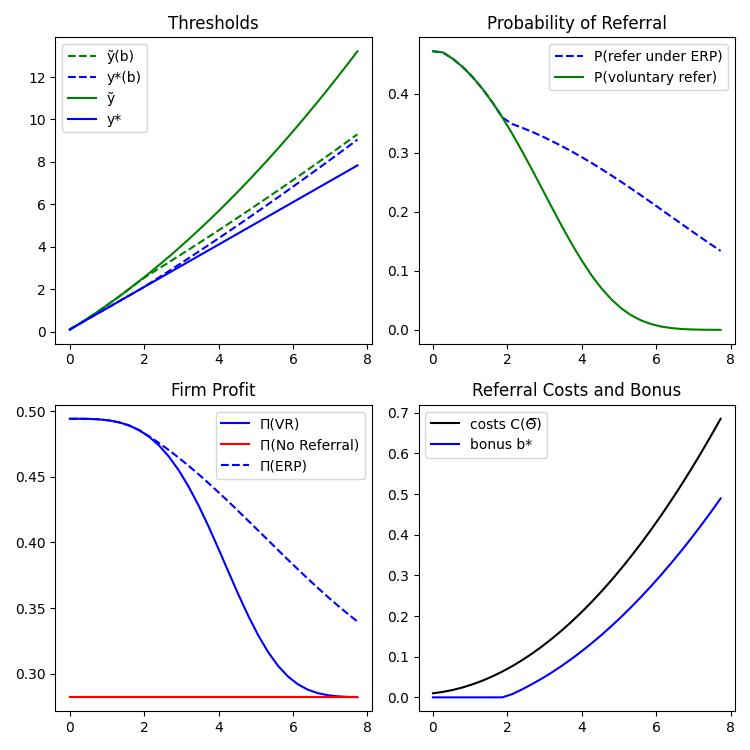
\includegraphics[width=12cm]{images/imperf_means_var.png}
    \centering
    \label{fig:mean_var}
\end{figure}

Figure \ref{fig:mean_var} illustrates the changes in the aforementioned variables of the model as the average general ability level of the workers, denoted as $\bar{\theta}$, varies from 0 to 8. Other model parameters are held constant at the following fixed values: the standard deviation of the general ability level is $\sigma = 1$, the correlation between workers is $\rho = 0.5$, and the social preference parameter is $\psi_{ij} = 0.5$.

As shown in Figure \ref{fig:mean_var}, under the given parameters, introducing an employee referral program makes sense for the firm when the average level of the workers' general ability is higher than 2. While the overall profit of the firm decreases with the average level of worker's general ability, the introduction of an ERP helps to mitigate this decrease caused by the decreasing probability of referral, and it extracts additional profits compared to the case of voluntary referrals. It is worth noting that the optimal bonus the firm pays to the referring worker is always lower than her referral costs.

\begin{figure}[ht]
    \caption{Changes in model variables as standard deviation of general ability $\sigma$ varies}
    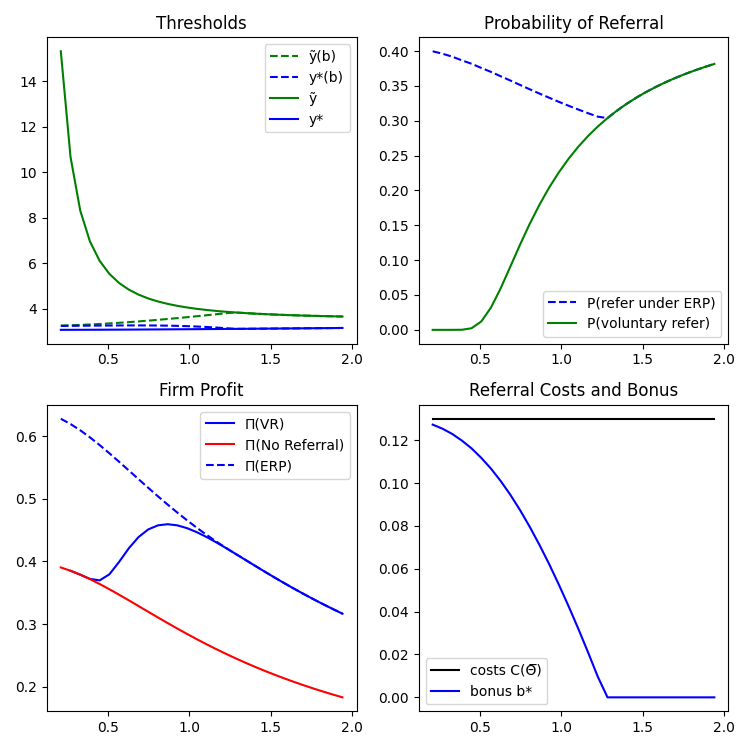
\includegraphics[width=12cm]{images/imperf_st_dev_var.png}
    \centering
    \label{fig:st_dev_var}
\end{figure}

Figure \ref{fig:st_dev_var} illustrates the changes in the  variables of the model as the standard deviation of the general ability of the workers, denoted as $\sigma$, varies from 0.2 to 2. Other model parameters are held constant at the following fixed values: the mean of the general ability level is $\bar{\theta} = 3$, the correlation between workers is $\rho = 0.5$, and the social preference parameter is $\psi_{ij} = 0.5$.

As shown in Figure \ref{fig:st_dev_var}, under the given parameters, introducing an employee referral program makes sense for the firm when the standard deviation of the general  ability of workers is lower than 1.25. The firm extracts larger benefits from voluntary referrals when there is a moderate variation in the general ability of the workers. However, the introduction of an employee referral program helps the firm increase its profit even when the variance of the general ability is low.

\begin{figure}[ht]
    \caption{Changes in model variables as correlation between workers $\rho$ varies}
    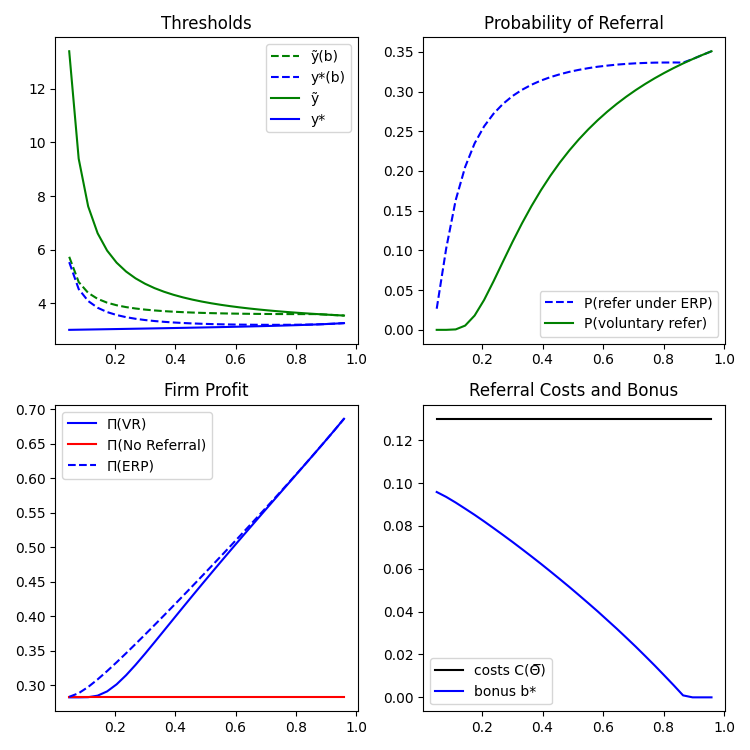
\includegraphics[width=12cm]{images/imperf_rho_var.png}
    \centering
    \label{fig:rho_var}
\end{figure}

Figure \ref{fig:rho_var} illustrates the changes in the  variables of the model as the correlation between workers, denoted as $\rho$, varies from 0.05 to 1. Other model parameters are held constant at the following fixed values: the mean of the general ability level is $\bar{\theta} = 3$, the standard deviation of the general ability level is $\sigma = 1$, and the social preference parameter is $\psi_{ij} = 0.5$. As shown in Figure \ref{fig:rho_var}, under the given parameters, introducing an employee referral program makes sense for the firm when the correlation between workers is lower than 0.85.

\begin{figure}[ht]
    \caption{Changes in model variables as social preference parameter $\psi_{ij}$ varies}
    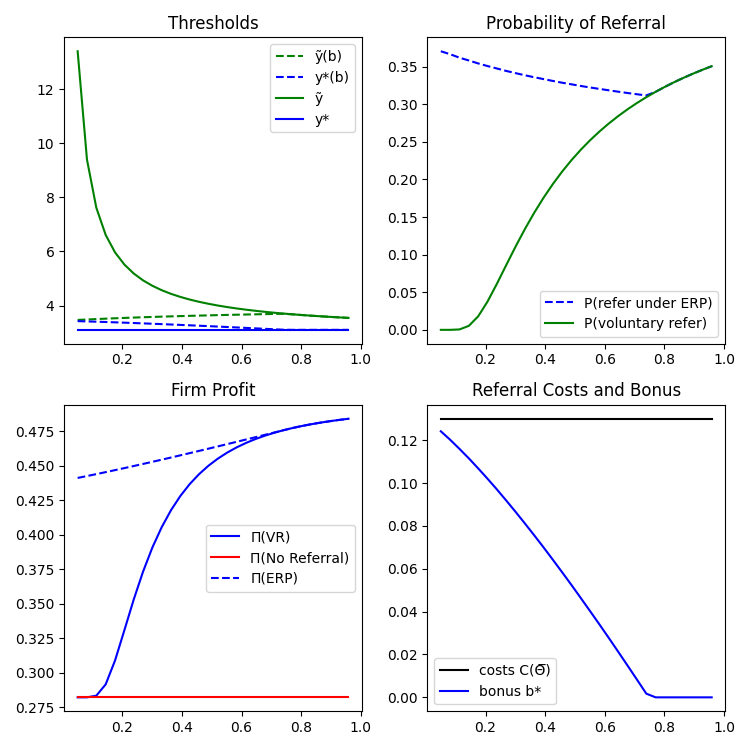
\includegraphics[width=12cm]{images/imperf_psi_var.png}
    \centering
    \label{fig:psi_var}
\end{figure}

Figure \ref{fig:psi_var} illustrates the changes in the  variables of the model as the social preference parameter, denoted as $\psi_{ij}$, varies from 0.05 to 1. Other model parameters are held constant at the following fixed values: the mean of the general ability level is $\bar{\theta} = 3$, the standard deviation of the general ability level is $\sigma = 1$, and the correlation between workers is $\rho = 0.5$. As shown in Figure \ref{fig:psi_var}, under the given parameters, introducing an employee referral program makes sense for the firm when the social preference parameter is lower than 0.72.

Figures \ref{fig:rho_var} and \ref{fig:psi_var} indicate that an ERP is most effective for weak ties between workers. Specifically, it helps maintain a high probability of referral when the intrinsic motivation of current employees is not sufficient for them to refer their contacts. Figure \ref{fig:psi_var} also shows that under the given parameters, the ERP works best for a low level of the social preference parameter $\psi_{ij}$. Meanwhile, Figure \ref{fig:rho_var} suggests that the additional benefits from referral when the correlation of workers is low are marginal. This result is intuitive because higher correlation between workers' abilities directly affects the firm's profit, whereas changes in the social preference parameter impact the firm's profit only through the threshold of current employees to refer their contacts and are thus less salient for the firm's profit.


\pagebreak

\end{document}